\documentclass[twoside,11pt]{article}
\usepackage{jair, theapa, rawfonts}
\usepackage[dvipsnames]{xcolor}
\usepackage{amsmath,amssymb,amsthm}
\usepackage[ruled,linesnumbered]{algorithm2e}
\usepackage{thmtools} 
\usepackage{booktabs}
\usepackage{paralist}
\usepackage{subcaption}
\usepackage{graphicx}
\usepackage{adjustbox}
\usepackage{multirow,array}

\usepackage[capitalise]{cleveref}
%\definecolor{vuborange}{rgb}{1.0,0.40,0.0}



%%%%%%
\newcommand\citet[1]{\citeauthor{#1}~[\citeyear{#1}]}

\newcommand\m[1]{\mathcal{#1}}



%% Theorems/Theory
\newtheorem{thm}{Theorem}
\newtheorem{definition}[thm]{Definition}
\newtheorem{prop}{Property}
\newtheorem{property}[prop]{Property}
\newtheorem{lem}{Lemma}
\newtheorem{lemma}[lem]{Lemma}
\newtheorem{propo}{Proposition}
\newtheorem{proposition}[propo]{Proposition}
\newtheorem{ex}{Example}
\newtheorem{example}[ex]{Example}
\newtheorem{theorem}[thm]{Theorem}


%% Comments
\newcommand\comment[1]{\marginpar{\tiny #1}}
\renewcommand\comment[1]{#1}
\newcommand{\tias}[1]{{\comment{\color{blue}Tias:#1}}}
\newcommand{\emilio}[1]{{\comment{\color{red}Emilio: #1}}}
\newcommand{\bart}[1]{{\comment{\color{green}Bart: #1}}}
\newcommand{\new}[1]{{\comment{{\color{blue} #1}}}}

%% Factoring
\newcommand\setstohit{\ensuremath{\m{H} }\xspace}
\newcommand\F{\ensuremath{\m{F} }\xspace}
\newcommand\subsetT{\ensuremath{\m{S} }\xspace}
\newcommand\bestsubsetT{\ensuremath{\m{S}_{best}}\xspace}
\newcommand\corrsetT{\ensuremath{\m{K} }\xspace}
\newcommand\setstohitall{\ensuremath{\m{H}_\mathit{all} }\xspace}
\newcommand\Iend{\ensuremath{I_\mathit{end} }\xspace}
\newcommand\formula{\ensuremath{\m{F} }\xspace}
\newcommand\formulac{\ensuremath{\m{C} }\xspace}
\newcommand\formulag{\ensuremath{\m{G} }\xspace}
\newcommand\mm[1]{\ensuremath{#1}\xspace}
\newcommand\nat{\mm{\mathbb{N}}}
\newcommand\ltrue{\mm{\textbf{t}}}
\newcommand\lfalse{\mm{\textbf{f}}}
\newcommand\uservars{\ensuremath{\m{U} }\xspace}
\newcommand\call[1]{\mm{\textsc{#1}}}
\newcommand\cohs{\mm{\call{CondOptHittingSet}}}
\newcommand\disjcorr{\mm{\call{DisjCorrSets}}}
\newcommand\sat{\texttt{{SAT}}\xspace}
\newcommand\grow{\mm{\call{Grow}}}
\newcommand\omus{\mm{\call{OUS}}}
\newcommand\comus{\mm{\call{OCUS}}}
\newcommand\disjmcs{\mm{\call{DisjointCorrectionSubsets}}}
\newcommand\omusinc{\mm{\call{OUS-Inc}}}
\newcommand\hitsetbased{hitting set--based\xspace} %en-dash!
\newcommand\satsets{\mm{\mathbf{SSs}}}
\newcommand\fall{\mm{\formula_{\mathit{all}}}}
\newcommand\algemilio[1]{\emilio{#1}\;}
\newcommand\UB{ub}
\newcommand\LB{lb}
\newcommand\maxsat{MaxSAT\xspace}
\newcommand\voc{\ensuremath{\Sigma}\xspace}
\newcommand\negset[1]{\mm{\overline{#1}}}


%%%%%
\newcommand\muses[1]{\ensuremath{\mathit{MUSs}(#1)}\xspace}
\newcommand\mcses[1]{\ensuremath{\mathit{MCSs}(#1)}\xspace}

%%%%%%%
\newcommand\onestep{\ensuremath{\call{Explain-One-Step}}\xspace}
\newcommand\parallelexplain{\ensuremath{\call{Parallel-One-Step-explain}}\xspace}
\newcommand\onestepo{\ensuremath{\call{Explain-One-Step-ocus}} \xspace}
\newcommand\iterativeonestep{\ensuremath{\call{Explain-One-Step-Iterative}}\xspace}

%%%%%%


\begin{document}
	
%%%%%%% ALGORITHM KEYWORDS
\SetKwInOut{Input}{Input}
\SetKwInOut{OptInput}{Optional}
\SetKwInOut{Output}{Output}
\SetKwInOut{State}{State}
\SetKwInOut{Ext.}{Ext}
\SetKwComment{command}{/*}{*/}
\SetKw{Break}{break}
%%%%%%%



\title{Efficiently }

\author{\name Emilio Gamba \email emilio.gamba@vub.be \\
       \name Bart Bogaerts \email bart.bogaerts@vub.be \\
       \addr Vrije Universiteit Brussel, Pleinlaan 5\\
       1050 Elsene, Belgium
       \AND
       \name Tias Guns \email tias.guns@vub.be \\
       \addr KULeuven, Oude Markt 13 - bus 5500,\\
       3000 Leuven, Belgium
   }

% For research notes, remove the comment character in the line below.
% \researchnote

\maketitle


\begin{abstract}

\end{abstract}

\begin{enumerate}
	\item Introduction
	\begin{itemize}
		\item Sequence of explanations for explaining the solutions of CSPs.
		\item Something explainability in artificial intelligence: workshops and conferences..
		\item unsatisfiability as a way to explain
		\item Something as followup work on our cosntraint satisfaction problems
	\end{itemize}
	\item Related works
	\begin{itemize}
		\item something about explanations and quality of the explanations 
		\item something about reviewing explanations for csps presented at IJCAI
		\item  somthing about weighted Unsatisfiable subsets
		\item  reviewing improvements that apply to unsatisfiable subsets
		\begin{itemize}
		\item  Abstract cores
		\item  Postponing optimisation
		\item  Disjoint MCS enumeration
		\item  something about incrementaltity (and more specifically) in maxsat solving
		\end{itemize}
		\item Seartching for explainable solutions in Sudoku 
	\end{itemize}
	\item Background
	\begin{itemize}
		\item Introduce MUSes/MCSes/Implciit HS ...
	\end{itemize}
	\item Motivation
	\begin{itemize}
		\item time to generate explanations too slow
		\item Require optimality
		\item Calls to OCUS very similar 		
	\end{itemize}
	\item OCUS
	\item Efficient OCUS computation for explanations
	
	\item Experiments
	\begin{itemize}
		\item RQ1. Cost comparison between MUS and Constrained for Logic Grid Puzzles+ Extra Demystify puzzles?
		\item RQ2. Domain-specific vs disj. mcs grow ?
		\item RQ3. Effect of COnstrainedness on the time required to computed explanations?
		\item RQ4. Does re-use of information across the different iterations improve efficiency? 
		\begin{itemize}
			\item testing OUSb incremental/OCUS incremental vs OUSb/OUS/OCUS
		\end{itemize}
		\item RQ5. Does appropriate sorting of literals lead to faster generation of individual explanations and explanation sequences:
		\begin{itemize}
			\item Iterative OUS vs rest
		\end{itemize} 
	\end{itemize}
	\item Conclusion and future work
	\item Acknowledgements
\end{enumerate}

\section{Introduction}
\label{sec:introduction}

\subsection{Contributions}
\label{sec:introduction}


Motivated by these observations, we develop algorithms that aid explaining CSPs and improve the state-of-the-art in the following ways: 
\begin{itemize}
	\item We develop algorithms that compute (cost-)\textbf{Optimal} Unsatisfiable Subsets (from now on called OUSs) based on the well-known hitting-set duality that is also used for computing cardinality-minimal MUSs \cite{ignatiev2015smallest,DBLP:conf/kr/SaikkoWJ16}.
	\item We observe that many of the individual calls for MUSs (or OUSs) can actually be replaced by a single call that searches for an optimal unsatisfiable subset \textbf{among subsets satisfying certain structural constraints}. In other words, we introduce the \emph{Optimal \textbf{Constrained} Unsatisfiable Subsets (OCUS)} problem and we show how $O(n^2)$ calls to MUS/OUS can be replaced by $O(n)$ calls to an OCUS oracle, where $n$ denotes the number of facts to explain. 
	\item We develop techniques for \textbf{optimizing} the O(C)US algorithms further, exploiting domain-specific information coming from the fact that we are in the \emph{explanation-generation context}. Such optimizations include the development of methods for \textbf{information re-use} between consecutive OCUS calls;
	\item We introduce an iterative algorithm that takes advantage of the cost of previously computed hitting sets and appropriate sorting on the literals-to-explain to reduce the time to generate an individual explanation as well as the whole explanation sequence.
	\item We improve the benchmark dataset of the experimental results by testing our approach on a larger number of CSPs and Weighted Unsatisfiable Instances.
\end{itemize}

\paragraph*{Publication history} This article is an extension of a previous paper presented at the International Joint Conference on Artificial Intelligence 2021 \cite{ijcai2021}.

\section{Related Works}
\label{sec:related-works}


\cite{bjornssonsearching} take a heuristic-search based approach to generate explanation sequences for Constraint Satisfaction problems with a use case on Sudoku puzzles. In that work, the quality of an explanation sequence is measured by a cost function associated with the strategy used, the number of times it is applied and the number of moves it derives.
% Survey paper: Explnaation in Constraint Satisfaction : A survey
In \cite{surveycsp2021}, \citeauthor{surveycsp2021} survey the important solver-agnostic \cite{junker2001quickxplain,ignatiev2015smallest,felfernig2012efficient} and solver-specific methods for generating explanations in Constraint Satisfaction in an effort to %(unify)
connect diverging research directions (Boolean Satisfiability, model-based diagnosis, constraint programming, quantified logics, and related areas). \emilio{cite some more ? and rephrase}

\section{Background}\label{sec:background}

We present all methods using propositional logic but our results easily generalize to richer languages, such as constraint languages, as long as the semantics is given in terms of a satisfaction relation  between expressions in the language and possible states of affairs (assignments of values to variables).

Let \voc be a set of propositional symbols, also called \emph{atoms}; this set is implicit in the rest of the paper. A \emph{literal} is an atom $p$ or its negation $\lnot p$. 
A clause is a disjunction of literals. A formula $\formula$ is a conjunction of clauses. 
Slightly abusing notation, a clause is also viewed as a set of literals and a formula as a set of clauses. We use the term clause and constraint interchangeably.

A (partial) interpretation $\m{I}$ is a consistent (not containing both $p$ and $\lnot p$) set of literals, for example $\{x_2,  \lnot x_3\}$. 
A \emph{model} of \formula is an interpretation that satisfies \formula; $\formula$ is said to be \emph{unsatisfiable} if it has no models.
\emilio{Write how satisfaction of a formula is defined}
Satisfaction of a formula \formula by an interpretation is defined as usual~\cite{faia/2009-185}.

A literal $l$ is a \emph{consequence} of a formula \formula if $l$ holds in all $\formula$'s models. 
In our running example, $\Iend = \{\lnot x_1, x_2,  \lnot x_3, x_4, \lnot x_5\}$ is the \emph{maximal consequence} that holds in all models and is also called the \emph{end interpretation}.
If $I$ is a set of literals, we write $\negset{I}$ for the set of literals $\{\lnot l\mid l\in I\}$.
For example, if we define $I_0 = \emptyset$ as the initial interpretation, then $\Iend \setminus I_0 = \{\lnot x_1, x_2,  \lnot x_3, x_4, \lnot x_5\}$ represents the remaining literals to derive and $\negset{\Iend \setminus I_0} = \{x_1, \lnot x_2,  x_3, \lnot x_4, x_5\}$ represents the complement of the remaining literals.

%\subsection{Properties and definitions}
In the following, we introduce key properties on unsatisfiable subsets on which we build our algorithms.

\begin{definition}
	A \emph{Minimal Unsatisfiable Subset} (MUS) of 
	\F is an unsatisfiable subset $\m{S}$ of $\F$ for which every strict subset of $\m{S} $ is satisfiable. 
	\muses{\F} denotes the set of MUSs of \F. 
\end{definition}


\begin{definition}
	A set $\m{S} \subseteq \formula$ is a \emph{Maximal Satisfiable Subset} (MSS) of $ \formula$ if $\m{S}$ is satisfiable and for all $\m{S}'$ with $\m{S}  \subsetneq  \m{S}'\subseteq\formula $, $\m{S}'$ is unsatisfiable.
\end{definition}

\begin{definition}
	A set $\m{S} \subseteq \formula$ is a \emph{correction subset} of \formula if $\formula\setminus\m{S}$ is satisfiable. 
	Such a $\m{S}$ is a \emph{minimal correction subset} (MCS)  of \formula if no strict subset of $\m{S}$ is also a correction subset. 
	\mcses{\F} denotes the set of MCSs of \F. 
\end{definition}

Each  MCS of \formula is the complement of an MSS of \formula and vice versa. 

\begin{definition}\label{def:minimal-hs}
	Given a collection of sets $\m{H}$, a hitting set of $\m{H}$ is a set $h$ such that  $h \cap C \neq \emptyset$ for every $C \in \m{H}$. A hitting set is \emph{minimal} if no strict subset of it is also a hitting set.
\end{definition}


The next proposition is the well-known hitting set duality \cite{DBLP:journals/jar/LiffitonS08,ai/Reiter87}  between MCSs and MUSs that forms the basis of our algorithms, as well as algorithms to compute MSSs \cite{DBLP:conf/sat/DaviesB13} and \emph{cardinality-minimal} MUSs \cite{ignatiev2015smallest}.

\begin{proposition}\label{prop:MCS-MUS-hittingset}
   
	A set  $\m{S} \subseteq \formula$ is an MCS of $ \formula$ iff  it is a \emph{minimal hitting set} of \muses{\formula}.
	A set  $\m{S} \subseteq \formula$ is a MUS of $ \formula$ iff  it is a \emph{minimal hitting set} of \mcses{\formula}.
\end{proposition}

	%	The formula \formula is thus: 
	%	\begin{description}
	%		\item[$\formula$] $\triangleq \formulac \wedge \m{I} \wedge \{\lnot \ell \}$ 
	%		\begin{itemize}
	%			\item $\formula(x_1) \triangleq \{ c_1 \wedge c_2 \wedge c_3\wedge c_4 \wedge \{\lnot x_1\}\}$
	%			\item $\formula(\lnot x_2) \triangleq \{ c_1 \wedge c_2 \wedge c_3\wedge c_4 \wedge \{x_2\}\}$
	%			\item $\formula(x_3) \triangleq \{ c_1 \wedge c_2 \wedge c_3\wedge c_4 \wedge \{\lnot x_3\}\}$
	%		\end{itemize}
	%		\item[$\formula_{incr}$] $\triangleq \formulac \wedge {\color{OliveGreen} (\Iend \setminus \ell)} \wedge {\color{Maroon} \{\lnot \ell \} }$ 
	%		\begin{itemize}
	%			\item $\formula_{incr}(x_1) \triangleq \{ c_1 \wedge c_2 \wedge c_3\wedge c_4 \wedge {\color{OliveGreen} \{\lnot x_2\}\wedge \{x_3\}} \wedge {\color{Maroon} \{\lnot x_1\} } \}$
	%			\item $\formula_{incr}(\lnot x_2) \triangleq\{ c_1 \wedge c_2 \wedge c_3\wedge c_4 \wedge {\color{OliveGreen} \{ x_1 \} \wedge \{x_3\}} \wedge {\color{Maroon} \{x_2\} } \}$
	%			\item $\formula_{incr}(x_3) \triangleq\{ c_1 \wedge c_2 \wedge c_3\wedge c_4 \wedge {\color{OliveGreen} \{ x_1 \}  \wedge \{\lnot x_2\}} \wedge {\color{Maroon} \{\lnot x_3\} }\}$
	%		\end{itemize}
	%		\item[$\formula_{incr, constr}$] $\triangleq \formulac \wedge {\color{OliveGreen} \Iend} \wedge {\color{Maroon} \overline{(\Iend\setminus I)}}$
	%		\begin{itemize}
	%			\item $\formulac\land \Iend \land \overline{(\Iend\setminus I)} = \{ c_1 \wedge c_2 \wedge c_3\wedge c_4\wedge {\color{OliveGreen} \{x_1\}\wedge\{\lnot x_2\} \wedge  \{x_3\} } \wedge {\color{Maroon}  \{\lnot x_1\} \wedge \{x_2\}\wedge \{\lnot x_3\} } \}$
	%			\item 	We define $p\triangleq$ \textit{exactly-one$(\{\lnot x_1, x_2, \lnot x_3\})$} and $f = \sum w_i \cdot c_i$ with clause weights $w_1 = 60, w_2=60, w_3=100, w_4=100, w_5=\infty, w_6=\infty, w_7=\infty, w_8=1, w_9=1, w_{10}=1$.
	%		\end{itemize}
	%		
	%	\end{description}
	%	% 	 Given \formulac, $f$, $\m{I}$ and $\Iend$ we have an OCUS-call with
	%	
	%	
	%	\begin{table}[!h]
	%		\centering
	%		\begin{tabular}{lcccc} 
	%			1&$\m{S}$ & $\sat(\m{S})$ & \grow($\m{S}$, $\formula$) & $\{  \formula \setminus \m{S}\}$\\ 
	%			\toprule[2pt]
	%			2& $\{\}$ & $True$ & $\{c_1 \wedge c_2 \wedge c_3 \wedge c_4 \wedge c_5 \wedge c_6 \wedge c_7\}$ & $\{c_8 \wedge c_9 \wedge c_{{10}}\}$ \\\midrule
	%			3& $\{c_9\}$ & $True$ & $\{c_1 \wedge c_2 \wedge c_3 \wedge ~c_4 \wedge c_5 \wedge c_9 \wedge c_7\}$ & $\{c_4 \wedge c_8 \wedge c_6 \wedge c_{{10}}\}$ \\\midrule
	%			4& $\{c_8\}$ & $True$ & $\{c_1 \wedge c_2 \wedge ~c_3 \wedge c_4 \wedge c_8 \wedge c_6 \wedge c_7\}$ & $\{c_3 \wedge c_5 \wedge c_9 \wedge c_{{10}}\}$ \\\midrule
	%			5& $\{c_{{10}}\}$ & $True$ & $\{c_1 \wedge c_2 \wedge ~c_3 \wedge c_4 \wedge c_8 \wedge c_6 \wedge c_{{10}}\}$ & $\{c_3 \wedge c_5 \wedge c_9 \wedge c_7\}$ \\\midrule
	%			6& $\{c_3 \wedge c_{{10}}\}$ & $True$ & $\{c_1 \wedge ~c_2 \wedge c_3 \wedge c_4 \wedge c_5 \wedge c_6 \wedge c_{{10}}\}$ & $\{c_2 \wedge c_8 \wedge c_9 \wedge c_7\}$ \\\midrule
	%			7& $\{c_4 \wedge c_9\}$ & $True$ & $\{c_1 \wedge c_2 \wedge ~c_3 \wedge c_4 \wedge c_8 \wedge c_9 \wedge c_{{10}}\}$ & $\{c_3 \wedge c_5 \wedge c_6 \wedge c_7\}$ \\\midrule
	%			8& $\{c_3 \wedge c_8\}$ & $False$ & $\{\}$ & $\{\}$ \\ \midrule
	%			
	%		\end{tabular}
	%		\caption{Step 1}
	%		\label{tab:explanation-steps-expanded}
	%	\end{table}
	%	%	\[\formula= \formulac\land \Iend \land \overline{(\Iend\setminus I)} = \{ c_1 \wedge c_2 \wedge c_3\wedge c_4\wedge c_5\wedge c_6\wedge c_7  \text{ \color{red} \sout{$\wedge c_8$}} \wedge c_9\wedge c_{10}\}\]
	%	
	%	%
	%	%$w_1 = 60, w_2=60, w_3=100, w_4=100, {\color{red}w_5=1}, w_6=\infty, w_7=\infty, {\color{red}w_8=\infty}, w_9=1, w_{10}=1$.
	%	\begin{table}[!h]
	%		\centering
	%		\begin{tabular}{lcccc} 
	%			&$\m{S}$ & $\sat(\m{S})$ & \grow($\m{S}$, $\formula$) & $\{  \formula \setminus \m{S}\}$\\ 
	%			\toprule[2pt]
	%			8& $\{c_2 \wedge c_5 \wedge c_{{10}}\}$ & $True$ & $\{~c1 \wedge c_2 \wedge c_3 \wedge c_4 \wedge c_5 \wedge c_9 \wedge c_{{10}}\}$ & $\{c_1 \wedge c_6 \wedge c_7\}$ \\\midrule
	%			9& $\{c_1 \wedge c_2 \wedge c_5 \wedge c_{{10}}\}$ & $False$ & $\{\}$ & $\{\}$ \\ \midrule
	%			
	%		\end{tabular}
	%		\caption{Step 2}
	%		\label{tab:explanation-steps-expanded}
	%	\end{table}
	%	%\[\formula= \formulac\land \Iend \land \overline{(\Iend\setminus I)} = \{ c_1 \wedge c_2 \wedge c_3\wedge c_4\wedge c_5\wedge c_6\wedge c_7  \text{ \color{red} \sout{$\wedge c_8$}} \wedge c_9\wedge \text{ \color{red} \sout{$\wedge c_{10}$}}\}\]
	%	%$w_1 = 60, w_2=60, w_3=100, w_4=100, {\color{green}w_5=1}, w_6=\infty, {\color{green}w_7=1}, {\color{red}w_8=\infty}, w_9=1, {\color{red}w_{10}=\infty}$.
	%	\begin{table}[!h]
	%		\centering
	%		\begin{tabular}{lcccc} 
	%			&$\m{S}$ & $\sat(\m{S})$ & \grow($\m{S}$, $\formula$) & $\{  \formula \setminus \m{S}\}$\\ 
	%			\toprule[2pt]
	%			10& $\{c_4 \wedge c_9 \wedge c_7\}$ & $False$ & $\{\}$ & $\{\}$ \\ \midrule
	%			
	%		\end{tabular}
	%		\caption{Step 3}
	%		\label{tab:explanation-steps-expanded}
	%	\end{table}
	%	


\section{Motivation}

Our work is motivated by the problem of explaining satisfaction problems through a sequence of simple explanation steps. This can be used to teach people problem-solving skills, to compare the difficulty of related satisfaction problems (through the number and complexity of steps needed), and in human-computer solving assistants.

Our original explanation generation algorithm \cite{ecai/BogaertsGCG20} starts from a formula $\formulac$ (in the application coming from a high level CSP), a partial interpretation $I$ (here also viewed as a conjunction of literals) and a cost function $f$ quantifying the difficulty of an explanation step, by means of a weight for every clause and literal in \formula. 

\begin{algorithm}[!h]
	\DontPrintSemicolon
	\caption{$\onestep(\formulac,f,I,\Iend)$}
	\label{alg:oneStep}
	$X_{best} \gets \mathit{nil}$\;
	\For{$l \in \{\Iend \setminus I\}$}{
		$X \gets \call{MUS}{(\formulac \land I \land \neg l)}$\;
		\If{$f(X)<f(X_{best})$\label{alg:oneStep:ifcheck}}{
			$X_{best} \gets X$\;
		}
	}
	\Return{$X_{best}$} 
\end{algorithm}

The goal is to find a sequence of \textit{simple} explanation steps, where the simplicity of a step is measured by the total cost of the elements used in the explanation.
An explanation step is an implication $I' \wedge \formulac' \implies N$ where $I'$ is a subset of already derived literals, $\formulac'$ is a subset of constraints of the input formula $\formulac$, and $N$ is a set of literals entailed by $I'$ and $\formulac'$ which are not yet explained.

The key part of the algorithm is the search for the next best explanation, given an interpretation $I$ derived so far. 
\cref{alg:oneStep} shows the gist of how this was done.
It takes as input the formula \formulac, a cost function $f$ quantifying the quality of explanations, an interpretation $I$ containing all already derived literals in the sequence so far, and the interpretation-to-explain $\Iend$. 
To compute an explanation, this procedure iterates over the literals that are still to explain, computes for each of them an associated MUS and subsequently selects the lowest cost one from found MUSs.
The reason this works is because there is a one-to-one correspondence between MUSs of $\formulac \land I \land \neg l$ and so-called \emph{non-redundant explanation} of $l$ in terms of (subsets of) $\formulac$ and $I$~\cite{ecai/BogaertsGCG20}. 

Experiments have shown that such a MUS-based approach can easily take hours, especially when multiple MUS calls are performed to increase the chance of finding a good MUS, and hence that algorithmic improvements are needed to make it more practical \cite{bogaerts2021framework}. 
We see three main points of improvement, all of which will be tackled by our generic OCUS algorithm presented in the next section. 

\begin{itemize}
	\item First of all, since the algorithm is based on \call{MUS} calls, there is no guarantee that the explanation found is indeed optimal %don't use ``the best'' -> non-unique 
	(with respect to the given cost function). 
	Performing multiple MUS calls is only a heuristic that is used to circumvent the restriction that \textit{there are no algorithms for cost-based unsatisfiable subset \textbf{optimization}}. 
	\item Second, this algorithm uses \call{MUS} calls for every literal to explain separately. The goal of all these calls is to find a single unsatisfiable subset of $\formulac \land I \land \overline{(\Iend\setminus I)}$ that contains exactly one literal from $\overline{(\Iend\setminus I)}$. This begs the questions whether it is possible \textit{to compute a single (optimal) unsatisfiable subset \textbf{subject to constraints}}, where in our case, the constraint is to include exactly one literal from $\overline{(\Iend\setminus I)}$. 
	\item Finally, the algorithm that computes an entire explanation sequence makes use of repeated calls to \onestep and hence will solve many similar problems. This raises the issue of \textit{\textbf{incrementality}: can we re-use the computed data structures to achieve speed-ups in later calls?}
\end{itemize}

\section{Optimal Unsatisfiable Subsets?}



\section{Optimal Constraint Unsatisfiable Subsets}


The first two considerations from the previous section lead to the following definition. 

\begin{definition}
	Let $\formula$ be a formula, $f:2^{\formula} \to \nat$ a cost function and  $p$ a predicate $p: 2^{\formula}\to \{true,false\}$.  We call %a set $U\subseteq \formulag$ a \emph{$p$-constrained $f$-OUS} of \formulag ($(p,f)$-OUS) \tias{what with the OCUS name here?} \bart{I propsoe to say. We call 
	$\m{S} \subseteq \formula$ an OCUS of \formula (with respect to $f$ and $p$) if \begin{itemize}                                      
		\item $\m{S}$ is unsatisfiable,
		\item $p(\m{S})$ is true
		\item all other unsatisfiable $\m{S}'\subseteq \formula$ for which $p(\m{S}')$ is true satisfy $f(\m{S}')\geq f(\m{S})$.
	\end{itemize}
\end{definition}


If we assume that the predicate $p$ is specified itself as a CNF over (meta)-variables indicating inclusion of clauses of $\m{F}$, and $f$ is obtained by assigning a weight to each such meta-variable, then the complexity of the problem of finding an OCUS is the same as that of the SMUS (cardinality-minimal MUS) problem  \cite{ignatiev2015smallest}: the associated decision problem is $\Sigma^P_2$-complete. Hardness follows from the fact that SMUS is a special case of OCUS, containment follows - intuitively - from the fact that this can be encoded as an $\exists\forall$-QBF using a Boolean circuit encoding of the costs. 

When considering the procedure \onestep from the perspective of OCUS defined above, the task of the procedure  is to compute an OCUS of the formula $\formula := \formulac\land I\land \overline{\Iend\setminus I}$ with $p$ the predicate that holds for subsets  that contain exactly one literal of $\overline{\Iend\setminus I}$, see \cref{alg:oneStepOCUS}. 
%In the rest of this paper, we study (incremental) algorithms for computing an OCUS. 

%\emilio{why is the text formatting weird ? Due to the algorithm names ? }
In order to compute an OCUS of a given formula, we propose to build on the hitting set duality of \cref{prop:MCS-MUS-hittingset}. 
For this, we will assume to have access to a solver \cohs that can compute hitting sets of a given collection of sets that are \emph{optimal} (w.r.t.\ a given cost function $f$) among all hitting sets \emph{satisfying a condition $p$}. 
The choice of the underlying hitting set solver will thus determine which types of cost functions and constraints are possible. 
In our implementation, we use a cost function $f$ as well as a condition $p$ that can easily be encoded as linear constraints, thus allowing the use of highly optimized mixed integer programming (MIP) solvers. The \cohs formulation is as follows:
%\bart{should be minimize or -f}\emilio{adapted}
\begin{align*}
	\small
	minimize_S \quad & f(S) \\ 
	s.t. \quad & p(S) \\
	& sum(H) \geq 1, \quad &&\forall H \in \setstohit \\
	& s \in \{0,1\}, \quad &&\forall s \in S
\end{align*}
%\bart{This is not what the reviewers asked for! They asked for MIP models of our ``arbitrary objective functions''. A mip encoding of a generic hitting set problem with only some ``at least one'' constraints is not going to help us, I think. }
% well, its not arbitrary but linear, and it is a weighted sum; will have to do
%\bart{indeed, it is not arbitrary! But that's exactly the point: if we say ``we only support linear objective functions'', then that reviewers concern ``how will you encode this as MIP?'' is resolved. We simply did not say that in the prior work. In any case, the model also doesn't hurt and breaks text a bit... } 
where $S$ is a set of MIP decision variables, one for every clause in $\formula$. In our case, $p$ is expressed as $\sum_{s \in \overline{\Iend\setminus I}} s = 1$. 
%On top of that, the $p$ can be used to enforce that some constraints in \formula are hard constraints and should always be included in the hitting set. %make a distinction between hard constraints (those that \emph{must} be included in the OCUS), which can be useful in case constraints are reified using assumption literals, or to \emph{group} constraints that should be enabled/disabled simultaneously. 
%\emilio{not trivial at all!!! If I understand correctly C = Hard + indicator variables where p imposes constraints on not using the Hard, but only the indicator variables}
%\emilio{Added an example:}
%For example, when explaining logic grid puzzles, the cnf-translated hard constraints ($\mathcal{C}_{hard}$) are reified using assumption literals i.e weighted soft constraints ($\mathcal{C}_{soft}$). In that case, $\mathcal{C} = \mathcal{C}_{hard} \ \cup \ \mathcal{C}_{soft}$.
% When aiming to explain satisfaction problems in terms of the subset of constraints and literals needed to derive a new literal, the initial interpretation $I$ should consist of indicators literals for each (group of) constraint(s) as well as already known true literals. }
%\bart{Previous sentence instead of earlier ``indicator'' sentence?}
%
%In our application, 
$f$ is a weighted sum over the variables in $S$. For example, (unit) clauses representing previously derived facts can be given small weights and regular constraints can be given large weights, such that explanations are penalized for including constraints when previously derived facts can be used instead. %relevant facts are directly available.

\begin{algorithm}[!h]
	\DontPrintSemicolon
	
	\caption{$\onestepo(\formulac,f,I,\Iend)$}
	\label{alg:oneStepOCUS}
	$p \leftarrow$ exactly one of $\overline{\Iend\setminus I}$\;
	\Return{$\comus(\formulac\land I\land \overline{\Iend\setminus I}, f, p)$} 
\end{algorithm}
\begin{algorithm}[!h]
	\DontPrintSemicolon
	$\setstohit  \gets \emptyset$ \; %\label{omus-line1} 
	\While{true}{
		$\m{S} \gets \cohs(\setstohit,f,p) $  \;%\tcp*{\small Find \textb    $\setstohit  \gets \setstohit  \cup \{  \formula \setminus \F''\}$ \;
		% f{optimal} solution}
		% \tcp{\small set with all unique clauses from hitting set}
		%     (sat?, $\kappa$) $\gets$ \texttt{SatSolver}($hs$)\;
		% \tcp{If SAT, $\kappa$ contains the satisfying truth assignment}
		% \tcp{IF UNSAT, $hs$ is the OUS }
		\If{ $\lnot \sat(\m{S})$}{\label{alg:ocus-sat-check}
			\Return{$\m{S}$} \;
		}
		$\m{S} \gets  \grow(\m{S},\F) $ \label{line:grow}\;
		$\setstohit  \gets \setstohit  \cup \{  \formula \setminus \m{S}\}$ \;
	}
	\caption{$\comus(\formula,f,p)$ }
	\label{alg:comus}
\end{algorithm}
%\tias{H should be initialised in algo 3}

%\tias{I would not show the above one as it is rather vague \bart{I would disagree with the vagueness. It makes abstraction of several things (what is $p$? what is $f$? How is Grow and CondOptHS implemented? But in my opinion that is good, since it shows close relation to the basic OUS algo as well as illustrating what is really going on and modularity.}, but immediately rewrite it as Alg2 the singleStepExplain:}
%\bart{I would avoid that :-) That way we mix up ``how to compute constrained OUSs?'' with ``how to compute explanations using constrained OUSs?''. These are two different concerns. We should show that we also tackle the first .  That way, our new ``singlestepexplain2'' will also look a lot simpler than singleStepExplain1 (if we use one oracle call to cOUS}

%\begin{algorithm}[ht]
%  \caption{$\call{ExplainCSPcOUS}({\cal C},f)$}
%  \label{alg:explainCSPcOUS}
%$E \gets \langle \rangle$\;
%$I_{end} \gets optimalPropagate({\cal C})$\;
%$\formulag \gets {\cal C} \cup I_{end} \cup \overline{\Iend}$\;
%$\setstohit \gets \{\formulag \setminus \{{\cal C} \cup I_{end}\}\}$\;
%// preseeding\\
%\For{$l \in I_{end}:$}{
%  $\setstohit \gets \setstohit \cup \{\formulag \setminus \grow(-l,\formulag)\} $\;
%}
%$I \gets \emptyset$\;
%$p \gets \{$exactly one of $\overline{\Iend}$ in the hitting set$\}$\; %, none of $I_{end}$ can be in the hitting set$\}$\;
%
%\While{$I \neq I_{end}$}{
%	update $p$ such that none of $\{I_{end} \setminus I\}$ and none of $\bar{I}$ can be in the hitting set\;
%    $\m{S} \gets \comus(\formulag,f,p,\setstohit)$\;
%	$I_{\mathit{best}} \gets I\cap \m{S}$\;
%    ${\cal C}_{\mathit{best}}\gets{\cal C}\cap \m{S}$\;
%	$N_{\mathit{best}} \gets \{I_{end} \setminus I\} \cap optimalPropagate(\m{S}) $\;
%	add $\{I_{\mathit{best}} \wedge {\cal C}_{\mathit{best}} \implies N_{\mathit{best}}\}$ to $E$\;
%	$I \gets I \cup N_{\mathit{best}}$\; 
%  }
%\Return{E}\;
%\end{algorithm}
Our generic algorithm for computing OCUSs is depicted in \cref{alg:comus}. It combines the hitting set-based approach for MUSs of \cite{ignatiev2015smallest} with the use of a MIP solver for (weighted) hitting sets as proposed for maximum satisfiability \cite{DBLP:conf/sat/DaviesB13}. The key novelty is the ability to add structural constraints to the hitting set solver, without impacting the duality principles of \cref{prop:MCS-MUS-hittingset}, as we will show.

Ignoring \cref{line:grow} for a moment, 
the algorithm alternates calls to a hitting set solver with calls to a \sat oracle on a subset $\m{S}$ of $\formula$. 
In case the \sat oracle returns true, i.e., the subset $\m{S}$ is satisfiable, the complement of $\m{S}$ is a correction subset of $\m{F}$ and is added to \setstohit. %In this way, the hitting set size always grows   THIS IS PLAINLY UNTRUE. PLEASE DONT PUT THIS BAKC. and a hitting set $\m{S}$ will always be a subset of $\formula$.

%Similar to %OCUS 
As in the SMUS algorithm of \citet{ignatiev2015smallest}, our algorithm contains an (optional) call to \grow. 
% However, the grow is optional: ``\emph{one can avoid the computation of MCS $\m{C}$ and use any correction subset $\m{C}'$ s.t. $\m{C} \subseteq \m{C}'$... Therefore, the grow procedure can be skipped}''.
The purpose of the \grow is to expand a satisfiable subset of $\m{F}$ further, to find a smaller correction subset and as such find stronger constraints on the hitting sets. 
In our case, the calls for hitting sets will also take into account the cost ($f$), as well as the meta-level constraints ($p$); as such, it is not clear a priori which properties a good \grow function should have here.
% These extensions resulting in novel problems, and hence in this extended setting, we had to reconsider the question `what constitutes a good grow?'.
We discuss the different possible implementations of \grow later and evaluate their performance in \cref{sec:experiments}. For correctness of the algorithm, all we need to know is that it returns a satisfiable subset $\m{S}'$ of $\m{F}$ with $\m{S}\subseteq\m{S}'$.
%In our case, OCUS requires to account for the cost, as well as the meta-level constraints. One of the contributions of this work is experimentally validating that using cost-based grow heuristics significantly reduces the time to find an OCUS. To summarize, OCUS is based on implicit hitting set enu-meration, like the SMUS algorithm. The key differences with respect to SMUS are the use of a cost function and meta-
%constraints. These extensions resulting in novel problems and hence in this extended setting we had to reconsider the question “what constitutes a good grow?”
%
%Instead of directly adding the complement of $\m{S}$ to \setstohit as done by \citet{ignatiev2015smallest}, our algorithm includes a call to \grow, which extends $\m{S}$ into a larger subset of $\formula$ that is still satisfiable (if possible). 
%\bart{AGAIN: DOES IGNATIEV NOT HAVE A GROW? A reviewer also asked this. We anwsered the reviewer that he was right: ignatiev has a grow. 
%Emilio, please check the reviews, and definitely our response that no such things remain! We cannot claim that ignatiev does not grow, simply because they say it is optional. We discussed this many times already}
%%\tias{here base grow impls?} \bart{Your next sentence is enough for me here. Alternatively we can in one stentence say that we consider a greedy and a maxsat-based implementation? }
%We discuss the different possible implementations of \grow later and evaluate their performance in \cref{sec:experiments}.

Soundness and completeness of the proposal follow from the fact that all sets added to \setstohit are correction subsets, and \cref{thm:soundcomplete}, which states that what is returned is indeed a solution and that a solution will be found if it exists. 



\begin{theorem}\label{thm:soundcomplete}
	Let $\m{H}$ be a set of correction subsets of \formula. 
	If $\m{S}$ is a hitting set of $\m{H}$ that is $f$-optimal among the hitting sets of $\m{H}$ satisfying a predicate $p$, and  $\m{S}$ is unsatisfiable, then $\m{S}$ is an OCUS of $\formula$. 
	If  $\m{H}$ has no hitting sets satisfying $p$, then $\formula$ has no OCUSs.
\end{theorem}
\begin{proof}
	For the first claim, it is clear that $\m{S}$ is unsatisfiable and satisfies $p$. Hence all we need to show is $f$-optimality of $\m{S}$.
	If there would exist some other unsatisfiable subset $\m{S}'$ that satisfies $p$ with $f(\m{S}')\leq f(\m{S})$, we know that $\m{S}'$ would hit every minimal correction set of $\m{F}$, and hence also every set in $\m{H}$ (since every correction set is the superset of a minimal correction set).
	Since $\m{S}$ is $f$-optimal among hitting sets of $\m{H}$ satisfying $p$ and $\m{S}'$ also hits $\m{H}$ and satisfies $p$, it must thus be that $f(\m{S})=f(\m{S}')$. 
	%  
	
	The second claim immediately follows from \cref{prop:MCS-MUS-hittingset} and the fact that an OCUS is an unsatisfiable subset of $\formula$. 
\end{proof}
% 	We define $f = \sum w_i$ the weighted sum over the following clause weights $w_1 = 20, w_2=20, w_3=20, w_4=20, w_5=1, w_6=1, w_7=1$. with interpretation $\{x_1, \lnot x_2, x_3 \}$:
%\[ c_1 = \lnot x_1 \vee \lnot x_2 \vee x_3\] \[ c_2 = \lnot x_1 \vee  x_2 \vee x_3 \text{\hspace*{20pt}} c_3 = \lnot x_3 \vee \lnot x_2 \]
%	If we already know $I= \{x_1\}$ represented by $c_5$, then $\overline{\Iend\setminus I} = \{ x_2, \lnot x_3\}$ is defined by the clauses $c_6 \wedge c_7$:
%\[c_5 = x_1 \text{\hspace*{20pt}} c_6 = x_2 \text{\hspace*{20pt}} c_7 = \lnot x_3 \]
%We define $p\triangleq$ \textit{exactlyone($c_6$, $c_7$)} and $f = \sum w_i$ the weighted sum over the following clause weights $w_1 = 20, w_2=20, w_3=20, w_4=20, w_5=1, w_6=1, w_7=1$.
% 

Perhaps surprisingly, correctness of the proposed algorithm does \emph{not} depend on monotonicity properties of $f$ nor $p$. In principle, any (computable) cost function and condition on the unsatisfiable subsets can be used. In practice however, one is bound by limitations of the chosen hitting set solver.





%\begin{example}
%	Let $\formulac$ be a CNF formula over literals $x_1, .., x_5$ with the following ten clauses:
%	\[c_{1}:=x_{1} \vee x_{2} \qquad c_{2}:=\lnot x_{5} \vee x_{1} \qquad c_{3}:=\lnot x_{4} \vee \lnot x_{3} \vee \lnot x_{5} \qquad c_{4}:=x_{2} \vee x_{3} \vee x_{4} \]
%	\[	c_{5}:=\lnot x_{2} \vee x_{3} \vee x_{4} \qquad c_{6}:=\lnot x_{2} \vee \lnot x_{3} \vee x_{4} \qquad c_{7}:=\lnot x_{5} \qquad c_{8}:=x_{1} \vee \lnot x_{3} \vee \lnot x_{4} \]
%	\[c_{9}:=\lnot x_{1} \vee x_{2} \vee x_{4} \vee x_{5} \qquad c_{10}:=\lnot x_{1} \vee x_{5} \]
%\end{example}

\section{Efficient OCUS computation for explanations}

Algorithm~\ref{alg:comus} is generic and can also be used to find (unconstrained) \omus{}s, namely with a trivially true $p$.
However, its constrainedness property allows to remove the need to compute a MUS/\omus for every literal. This decreases the complexity of explanation sequence generation from $O(n^2)$ calls to MUS to $O(n)$ calls to OCUS, namely, once for every step in the sequence. 

We now discuss optimizations to the OCUS algorithm that are specific to explanation sequence generation, though they can also be used when other forms of domain knowledge are present. 
%In this section, we discuss optimizations to the basic algorithm to compute OCUSs. 
%While our optimizations are inspired by the explanation generation problem, and tailored to solving this as efficiently as possible, the ideas presented here can also 

\subsection{Incremental OCUS Computation.}
%While searching for unsatisfiable subsets satisfying structural constraints already greatly reduces the number of calls to the unsatisfiable subset oracle, i
Inherently, generating a sequence of explanations still requires as many OCUS calls as there are literals to explain. 
Indeed, a greedy sequence construction algorithm %high-level algorithm, not explicitly portrayed in the current paper, 
calls \onestepo iteratively with a growing interpretation $I$ until $I=\Iend$.

All of these calls to \onestepo, and hence OCUS, are done with very similar input (the set of constraints does not change, and the $I$ slowly grows between two calls). For this reason, it makes sense that information computed during one of the earlier stages can be useful in later stages as well. 

The main question is, suppose two \comus calls are done, first with inputs $\formula_1$, $f_1$, and $p_1$, and later with $\formula_2$, $f_2$, and $p_2$; how can we make use as much as possible of the data computations of the first call to speed-up the second call? The answer is surprisingly elegant. The most important data \comus keeps track of  is the collection \setstohit of correction subsets that need to be hit.

This collection in itself is not useful for transfer between two calls, since -- unless we assume that $\formula_2$ is a subset of $\formula_1$, there is no reason to assume that a set in $\setstohit_1$ should also be hit in the second call. 
However, each set $H$ in $\setstohit$ is the complement (with respect to the formula at hand) of a \emph{satisfiable subset} of constraints, and this satisfiability remains true. 
Thus, instead of storing $\setstohit$, we can keep track of a set \satsets of \emph{satisfiable subsets} (the sets $\m{S}$ in the \comus algorithm). 
When a second call to \comus is performed, we can then initialize $\setstohit$ as the complement of each of these satisfiable subsets with respect to $\formula_2$, i.e., \[\setstohit\gets \{\formula_2\setminus \m{S}\mid \m{S}\in \satsets\}.\]

The effect of this is that we \textit{bootstrap} the hitting set solver with an initial set $\setstohit$.

For hitting set solvers that natively implement incrementality, we can generalize this idea further: we know that all calls to $\comus(\formula,f,p)$ will be cast with $\formula \subseteq \m{C}\cup \Iend \cup \overline{\Iend \setminus I_0}$, where $I_0$ is the start interpretation. Since our implementation uses a MIP solver for computing hitting sets (see Section~\ref{sec:backgr}), and we have this upper bound on the set of formulas to be used, we can initialize all relevant decision variables once. To compute the conditional hitting set for a specific $\formulac\cup I\cup \overline{\Iend\setminus I} \subseteq \m{C}\cup \Iend \cup \overline{\Iend \setminus I_0}$ we need to ensure that the MIP solver only uses literals in $\formulac\cup I\cup \overline{\Iend\setminus I}$, for example by giving all other literals infinite weight in the cost function. In this way, the MIP solver will automatically maintain and reuse previously found sets-to-hit in each of its computations. 
% \emilio{need to re-read reviews, reviewers asked (?) for simple MIP model of the problem}
%\emilio{Maybe an introductory text?}
%\paragraph{Bounded OUS computation for efficient explanation-generation}
%1. Leg eerst uit he bounded OUS kan werken (gegeven een bound, stop als je HS hogere waarde heeft)
%2. Leg dan uit hoe je bounded OUS kan gebruiken in de lus
%3. Leg dan de optimalisatie met sorteren uit en waarom we dat doen (zie comments)
%\paragraph{Bounded OUS computation} The principle of reusing information from previous MUS/\omus calls can also be used when computing an \omus{} for every literal separately, more precisely in Algorithm~\ref{alg:oneStep} where MUS can be replaced by \omus. 
%\bart{What does replacing MUS by \omus have to do with reusing information? Nothing.}
%Furthermore \bart{This ``furthermore'' is the *only* ``reusing information'' we would do. Furthermore is not the right word for that}, we can push the check of line \ref{alg:oneStep:ifcheck} into the \omus call either by passing it directly to the hitting set solver if it accepts an upper bound $ub$ (like MIP solvers do); or by adding a condition on the found $\m{S}$ before the \sat call %at line \ref{alg:ocus-sat-check} of
%Algorithm~\ref{alg:comus} \bart{to explain how OCUS corresponds to OUS}, i.e interrupt this \omus-call if $f(\m{S}) > ub$.  \bart{This is very technical. This is \emph{how} we do something. What is missing is \emph{what} we want, namely a bounded OUS check.}
%Since the bounding on the \omus cost has the most effect if cheap \omus{}s are found early in the loop, we sort the literals based on their corresponding upper bound \bart{Which is? Where does it come from?} , initialized at $f(\formulac \land I_0 \land \overline{\Iend \setminus I_0})$.

\subsection{Domain-Specific Implementations of \grow.} \label{para:domainspecificgrow}
%In the context of explanations we are in, we have a way of generating large satisfiable subsets quite easily and hence we conjecture that implementing a domain-specific \grow will be more efficient than generic version of the \grow algorithm. 

The goal of the \grow procedure is to turn $\m{S}$ into a larger subformula of $\formula$. The effect of this is that the complement added to \setstohit will be smaller, and hence, a stronger restriction for the hitting set solver is found.  

Choosing an effective \grow procedure requires finding a difficult balance: on the one hand, we want our subformula to be as large as possible (which ultimately would correspond to computing the maximum satisfiable subformula), %to derive the most precise information we can get, 
but on the other hand we also want the procedure to be very efficient as it is called in every iteration. 

For the case of explanations we are in, we make the following observations: 
\begin{itemize}
	\item Our formula at hand (using the notation from the \onestepo algorithm) consists of three types of clauses: \begin{inparaenum}\item  (translations of) the problem constraints (this is \formulac) \item literals representing the assignment found thus far (this is $I$), and \item the negations of literals not-yet-derived (this is $\overline{\Iend\setminus I}$). \end{inparaenum}
	\item $\formulac$ and $I$ together are satisfiable, with assignment $I_{end}$, and \emph{mutually supportive}, by this we mean that making more constraints in \formulac true, more literals in $I$ will automatically become true and vice versa. 
	\item The constraint $p$ enforces that each hitting set will contain \textbf{exactly} one literal of  $\overline{\Iend\setminus I}$
\end{itemize}
Since the restriction on the third type of elements of $\formula$ are already strong, it makes sense to use the \grow($\m{S}$,$\F$) procedure to search for a \emph{maximal} satisfiable subset of $\formulac\cup I$ with hard constraints that $\m{S}$ should be satisfied, using a call to an efficient  (partial) \maxsat solver. Furthermore, we can initialize this call as well as any call to a \sat solver with the polarities for all variables set to the value they take in $\Iend$. %This is likely to lead to a fairly large satisfiable subset and hence a good correction set. 

We evaluate different grow strategies in the experiments section, including the use of partial \maxsat as well as weighted partial \maxsat based on the weights in the cost function $f$.

\subsection{Disjoint Minimum Correction Subsets enumeration}

\paragraph{Application to OCUS} Computing dijsoint mcses ensures diversification of sets-to-hit. It can be either applied as \begin{inparaenum}[(i)]
	\item a bootstrapping method for \ref{alg:comus} on line \ref{alg:ocus-line1} or
	\item a replacement for the \grow procedure on line \ref{alg:ocus:grow}. 
\end{inparaenum}


Inspired by \cite{marques2013computing}, 
\begin{itemize}
	\item Work similarly to \grow
	\item Initialisation of a maxsat solver with constraints as hard clauses
	\item Hitting set is also hard clause
	\item Remaining soft clauses is the current interpretation - hs
	\item Repeat: Compute maxsat solution, which is a satisfiable subset and its complement is added as a hard clause. If it's true in the satisfiable subset it's not going to be in its complement (the correction subset).
	\item Stops when no solutions can be found anymore.
\end{itemize}

\begin{algorithm}[!h]
	\DontPrintSemicolon
	\Output{$\m{K}$: Disjoint correction subsets}
	$\m{K} \gets \emptyset$ \label{alg:disjmcs:init} \;
	
	\While{$\sat(S)$}{
		$\m{S}' \gets  \grow(\m{S}, \formula)$\;
		$ \m{K} \gets \m{K} \cup \{\formula \setminus \m{S}'\}$\;
		$ \m{S} \gets \m{S}  \cup \m{S}'$\;	
	}
	\Return $\m{K}$
	\caption{$\disjmcs(\formula,\subsetT)$ }
	\label{alg:comus}
\end{algorithm}

The following example will be used as a running example to illustrate these and following concepts.

\begin{example}
	Let $\formulac$ be a CNF formula over variables $x_1, x_2, x_3$ with the following four clauses:
	\[ c_1 := \lnot x_1 \vee \lnot x_2 \vee x_3 \qquad  c_2 := \lnot x_1 \vee  x_2 \vee x_3\] \[  c_3 := x_1 \qquad c_4 := \lnot x_2 \vee \lnot x_3 \]
	
	\begin{itemize}
		\item $\Iend$, the final interpretation, is $\{x_1, \lnot x_2,  x_3\}$
		\item $\m{I}$, the current interpretation, is $\{ \emptyset \}$
		\item $\overline{\Iend\setminus I} =  \{\lnot x_1, x_2, \lnot x_3\}$.
	\end{itemize}
	 To define the input for the OCUS call, we add new clauses representing the final interpretation $\Iend$:
\[ c_5 := \{ x_1\}\qquad  c_6:=\{\lnot x_2\} \qquad  c_7 := \{ x_3\}\]
and the complement of the to-be-derived facts $\overline{\Iend\setminus I}$: 
\[ c_8 := \{\lnot x_1\}\qquad  c_9:=\{x_2\} \qquad  c_{10} := \{\lnot x_3\}\]
The formula \formula in the \comus-call is thus: 
% 	 Given \formulac, $f$, $\m{I}$ and $\Iend$ we have an OCUS-call with
\[\formula_{incr, constr}= \formulac\land \Iend \land \overline{(\Iend\setminus I)} = \{ c_1 \wedge ... \wedge c_{10}\}\]	

We define $p\triangleq$ \textit{exactly-one$(c_8, c_9, c_{10})$} and $f = \sum w_ic_i$ with clause weights \[w_1 = 60, w_2=60, w_3=100, w_4=100, w_5=\infty, w_6=\infty, w_7=\infty, w_8=1, w_9=1, w_{10}=1\]

\emph{In this example, the \grow we used is the one called \emph{Max-Actual-Unif} in \cref{sec:experiments}.}
\end{example}

\begin{table}[!h]
	\centering
%	\begin{adjustbox}{max width=\columnwidth}
		\begin{tabular}{lcccc} 
%			\bottomrule[2pt]
			\multicolumn{5}{c}{Step 1. Explanation of $x_1$: $c_3 \implies x_1$}\\
			\toprule[2pt]
			&$\m{S}$ & $\sat(\m{S})$ & \grow($\m{S}$, $\formula$) & $\setstohit  \gets \setstohit  \cup \{  \formula \setminus \m{S}\}$\\ 
			\toprule[2pt]
			1 & $\{ \lnot x_1\}$ & $\mathit{true}$ & $\{c_1, c_2, c_4, \lnot x_1, \lnot x_2, x_3 \}$ & $\{ \{c_3, x_1, x_2, \lnot x_3 \}\}$   \\
			\midrule	
			2 &$\{\lnot x_3\}$ & $\mathit{true}$ & $\{c_1 , c_2 , c_4, \lnot x_1 , \lnot x_2 ,  \lnot x_3 \}$ & $\{ \{c_3, x_1, x_2, \lnot x_3 \}, \{c_3, x_1 , x_2 , x_3 \}\}$  \\  
			\midrule
			\multirow{2}{*}{3} &\multirow{2}{*}{$\{x_2\}$} & \multirow{2}{*}{$\mathit{true}$} & \multirow{2}{*}{$\{c_1 , c_2 , c_3, x_1 , x_2 , x_3 \}$} & $\{ \{c_3, x_1, x_2, \lnot x_3 \}, \{x_1 , x_2 , x_3 , c_3 \}$  \\
			& & & & $\{ c_4, \lnot x_1 , \lnot x_2 , \lnot x_3\} \}$ \\
			\midrule
			\multirow{2}{*}{4} &\multirow{2}{*}{$\{x_2, c_4\}$} & \multirow{2}{*}{$\mathit{true}$} & \multirow{2}{*}{$\{  c_1 , c_2 , c_4, \lnot x_1 , x_2 , \lnot x_3\}$} & $\{ \{c_3, x_1, x_2, \lnot x_3 \}, \{x_1 , x_2 , x_3 , c_3 \}$  \\
			& & & & $\{\lnot x_1 , \lnot x_2 , \lnot x_3, c_4\}, \{x_1 , \lnot x_2 , x_3 , c_3 \}\}$ \\
			\midrule
			\multirow{3}{*}{5} &\multirow{3}{*}{$\{\lnot x_3, c_3\}$} & \multirow{3}{*}{$\mathit{true}$} & \multirow{3}{*}{$\{   c_1  , c_3 , c_4, x_1, \lnot x_2 , \lnot x_3 \}$} & $\{ \{c_3, x_1, x_2, \lnot x_3 \}, \{x_1 , x_2 , x_3 , c_3 \}$  \\
			& & & & $\{\lnot x_1 , \lnot x_2 , \lnot x_3, c_4\}, \{x_1 , \lnot x_2 , x_3 , c_3 \}$ \\
			& & & & $\{ c_2, \lnot x_1 , x_2 , x_3\}\}$ \\
			\midrule
			6 &$\{\lnot x_1, c_3\}$ & $\mathit{false}$ & $\emptyset$ & / \\
%			\bottomrule
			\\
			\multicolumn{5}{c}{Step 2. Explanation of $x_3$: $c_1 \wedge c_2 \wedge x_1 \implies x_3$}\\
			\toprule[2pt]
			\multirow{3}{*}{7} &\multirow{3}{*}{$\{x_1 , \lnot x_3 , c_2\}$} & \multirow{3}{*}{$\mathit{true}$} & \multirow{3}{*}{$\{   c_2 , c_3 , c_4,x_1 , x_2 , \lnot x_3 \}$} & $\{ \{c_3, x_1, x_2, \lnot x_3 \}, \{x_1 , x_2 , x_3 , c_3 \}$  \\
			& & & & $\{\lnot x_1 , \lnot x_2 , \lnot x_3, c_4\}, \{x_1 , \lnot x_2 , x_3 , c_3 \}$ \\
			& & & & $\{ c_2, \lnot x_1 , x_2 , x_3\}, \{c_1, \lnot x_2 , x_3 \} \}$ \\
			\midrule
			%		
			%		7 & $\{ x_1 , \lnot x_3 , c_2\}$ & $\mathit{true}$ & $\{ c_2 , c_3 , c_4,x_1 , x_2 , \lnot x_3 \}$ & $\{ ..., \{c1, \lnot x2 , x3 \}\}$  \\ \midrule
			8 &$\{ x_1 , \lnot x_3 , c_1 , c_2 \}$ & $\mathit{false}$ & $\emptyset$ & / \\
%			\bottomrule
			\\
			\multicolumn{5}{c}{Step 3. Explanation of $\lnot x_2$: $c_4 \wedge x_3 \implies \lnot x_2$}\\
			\toprule[2pt]
			9 &$\{ x_2 , x_3, c_4 \}$ & $\mathit{false}$ & $\emptyset$ & / \\
			
		\end{tabular}
%	\end{adjustbox}
	\caption{Sequence of explanation generated with \onestepo}
	\label{tab:explanation-steps-expanded:step1}
\end{table}
%
%\begin{table}[!h]
%	\centering
%	%	\begin{adjustbox}{max width=\columnwidth}
%	\begin{tabular}{lcccc} 
%		&$\m{S}$ & $\sat(\m{S})$ & \grow($\m{S}$, $\formula$) & $\setstohit  \gets \setstohit  \cup \{  \formula \setminus \m{S}\}$\\ 
%		\toprule[2pt]
%		\multirow{3}{*}{7} &\multirow{3}{*}{$\{x_1 , \lnot x_3 , c_2\}$} & \multirow{3}{*}{$\mathit{true}$} & \multirow{3}{*}{$\{   c_2 , c_3 , c_4,x_1 , x_2 , \lnot x_3 \}$} & $\{ \{c_3, x_1, x_2, \lnot x_3 \}, \{x_1 , x_2 , x_3 , c_3 \}$  \\
%		& & & & $\{\lnot x_1 , \lnot x_2 , \lnot x_3, c_4\}, \{x_1 , \lnot x_2 , x_3 , c_3 \}$ \\
%		& & & & $\{ c_2, \lnot x_1 , x_2 , x_3\}, \{c_1, \lnot x_2 , x_3 \} \}$ \\
%			\midrule
%%		
%%		7 & $\{ x_1 , \lnot x_3 , c_2\}$ & $\mathit{true}$ & $\{ c_2 , c_3 , c_4,x_1 , x_2 , \lnot x_3 \}$ & $\{ ..., \{c1, \lnot x2 , x3 \}\}$  \\ \midrule
%		8 &$\{ x_1 , \lnot x_3 , c_1 , c_2 \}$ & $\mathit{false}$ & $\emptyset$ & / \\
%		\bottomrule
%	\end{tabular}
%	%	\end{adjustbox}
%	\caption{Step 2. \comus Incremental Explanation of $x_3$ ($c_1 \wedge c_2 \wedge x_1 \implies x_3$)}
%	\label{tab:explanation-steps-expanded:step2}
%\end{table}
%
%\begin{table}[!h]
%	\centering
%	%	\begin{adjustbox}{max width=\columnwidth}
%	\begin{tabular}{lcccc} 
%		&$\m{S}$ & $\sat(\m{S})$ & \grow($\m{S}$, $\formula$) & $\setstohit  \gets \setstohit  \cup \{  \formula \setminus \m{S}\}$\\ 
%		\toprule[2pt]
%		9 &$\{ x_2 , x_3, c_4 \}$ & $\mathit{false}$ & $\emptyset$ & / \\
%		\bottomrule
%	\end{tabular}
%	\caption{Step 3. \comus Incremental Explanation of $\lnot x_2$ ($c_4 \wedge x_3 \implies \lnot x_2 $)}
%	\label{tab:explanation-steps-expanded:step1}
%\end{table}





\paragraph{Example 1 (cont.)} 
%Consider line 0 in table \ref{tab:explanation-steps-expanded}. During the \grow procedure, the \maxsat solver \emph{Max-Actual-Unif} with polarities set to \Iend branches when multiple assignment to a literal are possible. By hinting the polarities of the literals, we guide the solver and it assigns all values according to the end interpretation and neither $c_6$ nor $c_7$ is taken.



\subsection{Explanations with Bounded OUS.}
%Context: how to do OUS 

The cost of an Optimal Unsatisfiable Subset for a literal in the unconstrained version is bounded by a lower bound and an upper bound. 
\begin{description}
	\item[Initialization] The lower bound is initialized at 0. 
	\begin{itemize}
		\item[$>$] The lower bound can be improved by computing an \emph{optimal} hitting set on the disjoint minimum correction subsets present of the current formula $\formula$ to explain.			
	\end{itemize}
	\item[Update] Updated at every iteration by the cost of a computed optimal \emph{Hitting set}.
	\item[Use] 
	\begin{itemize}
		\item[$>$] If an Optimal Unsatisfiable Subset is found, then its cost can be used as an upper bound on the cost of a subsequent OUS.
		\item[$>$] The \textbf{LB} helps in sorting the literals according to the current cost of the least-cost \emph{Hitting Set} computed so far.		
	\end{itemize}
\end{description}


Instead of working \comus-based, we can now also generate optimal explanations by replacing the MUS call by an \omus call  in Algorithm~\ref{alg:oneStep} (where OUS is computed as in Algorithm~\ref{alg:comus}, but with a trivially true $p$). 
%Observation: waste of time
When doing this, we know that every \comus of cost greater than or equal to $f(X_{\mathit{best}})$ will be discarded by the check on Line 4 of Algorithm~\ref{alg:oneStep}.
%Optimizatino: what do we do? 
As such, a next optimization is to, instead of searching for an OUS, perform a \emph{bounded OUS check}, which only computes an OUS in case one of cost smaller than a given bound $\mathit{ub}$ exists.  
%Detail: how do we do it? 
In our specific implementation, bounded \omus is performed by interrupting this \omus-call (after Line 3 Algorithm~\ref{alg:comus}) if $f(\m{S}) > \mathit{ub}$.

Since the bounding on the \omus cost has the most effect if cheap \omus{}s are found early in the loop across the different literals, we keep track of an upper bound of the cost of an OUS for each literal to explain. This is initialized to a value greater than any \omus, e.g., as $f(\formulac \land I_0 \land \overline{\Iend \setminus I_0})$, and is updated every time an \omus explaining that literal is found; when going through the loop in Line 2 of Algorithm~\ref{alg:comus}, we then handle literals in order of increasing upper bounds.

\subsection{Iterative searching for \omus}



\begin{algorithm}[!h]
	\DontPrintSemicolon
	\tcp{Initilisation of Heap with tuples $\langle $cost$, $ literal$, $ hs$ \rangle$}
	$lb \gets$ \texttt{heap()}\;
	\ForEach{$\ell \in  (\Iend \setminus I)$}{
		$	\formula_{\ell} \gets  \formulac \wedge (\Iend \setminus \ell) \wedge \{\lnot \ell \}$ \;
		$ \setstohit_{\ell} \gets \emptyset $\; 
		\texttt{lb.push($\langle 0, \ell, \emptyset \rangle $)}\;
	}
	\tcp{\comus loop}
	\While{$true$}{
		
		$(cost, \ell, \m{S}) \gets$\texttt{lb.pop()} \tcp*{Literal with lowest bound}
		
		\If{ $\lnot \sat(\m{S})$}{
			\Return{$\m{S}$} \tcp*{\color{Green}OCUS found}
		}
		
		$\m{S} \gets  \grow(\m{S}, 	\formula_{\ell})$ \tcp*{Hitting set grown to a Satisfiable Subset}
		
		$\setstohit_{\ell}  \gets \setstohit_{\ell}  \cup \{  \formula_{\ell} \setminus \m{S}\}$ \tcp*{Correction Subset added to sets-to-hit}
		
		$\m{S} \gets \cohs(\setstohit_{\ell},f,p)$ \tcp*{Optimal hitting set}
		
		\texttt{lb.push($\langle f(\m{S}), \ell, \m{S} \rangle$)}\;
	}
	\caption{$\iterativeonestep(\formulac,f,I, \Iend)$}
	\label{alg:iterative_ocus}
\end{algorithm}






Algorithm \ref{alg:comus} computes an \comus for a given $\formula$, cost function $f$, and predicate $p$. 


% \todo{``old maxsat'' comes here}






%
%
%The main problems of this algorithm are:
%\begin{enumerate}
%	\item It does not take advantage of the repeated calls on similar incremental formulas, where the problem constraints remain the same, but the partial interpretation $\m{I}$ increases in size.
%%	\item The ordering of the expl$ained literals highly impacts the total execution time.
%\end{enumerate}

%Therefore we introduce 3 notions: 
%\begin{description}
%	\item[Incrementality (incr)] Re-use of information between successive MUS-calls.
%	\item[Constrainedness (constr)] Instead of computing the explanation for every literal separately, we find a single unsatisfiable subset of $\formulac \wedge \Iend \wedge \overline{(\Iend\setminus I)}$ that contains exactly one literal from $\overline{(\Iend\setminus I)}$.
%	\item[Iterative search] Step-wise and iterative search towards best explanation based on bounded cost.
%\end{description}


The CNF formulas are the following:

\begin{description}
	\item[$\formula$ $\triangleq \formulac \wedge \m{I} \wedge \{\lnot \ell \}$] 
	\item[$\formula_{constr}$ $\triangleq \formulac \wedge \m{I} \wedge \overline{(\Iend\setminus I)}$] \textit{Formula under partial interpretation $\m{I}$ over constrained subset of variables $\overline{(\Iend\setminus I)}$.}
	\item[$\formula_{incr}$ $\triangleq \formulac \wedge (\Iend \setminus \ell) \wedge \{\lnot \ell \}$] \textit{Formula under incremental partial interpretation $\m{I}$}
	\item[$\formula_{incr, constr}$ $\triangleq \formulac \wedge \Iend \wedge \overline{(\Iend\setminus I)}$] \textit{Formula under incremental partial interpretation $\m{I}$ over constrained subset of variables $\overline{(\Iend\setminus I)}$.}
\end{description}

%	\item[UB] \emph{An upper bound} on the cost of the next cheapest/best \omus
%	\begin{description}
%		 \item[Initialization] The upper bound is initialized as cost of the formula $\formula$ to explain $f(\formula)$.
%		 \item[Update] Improved whenever an \emph{OUS} for that given literal is found
%		 \item[Use] The smallest \textbf{UB} among all remaining literals to explain bounds the cost of the next \omus and is thus used to interrupt the \omus computation if the cost of the current hitting set exceeds the smallest \textbf{UB}.
%	\end{description}


%\section{Additional optimizations}
\clearpage
\section{Experimental Results}\label{sec:experiments}

\subsection{RQ1. Cost comparison between MUS and Constrained for Logic Grid Puzzles+ Extra Demystify puzzles}
\begin{figure}[h]
	\centering
	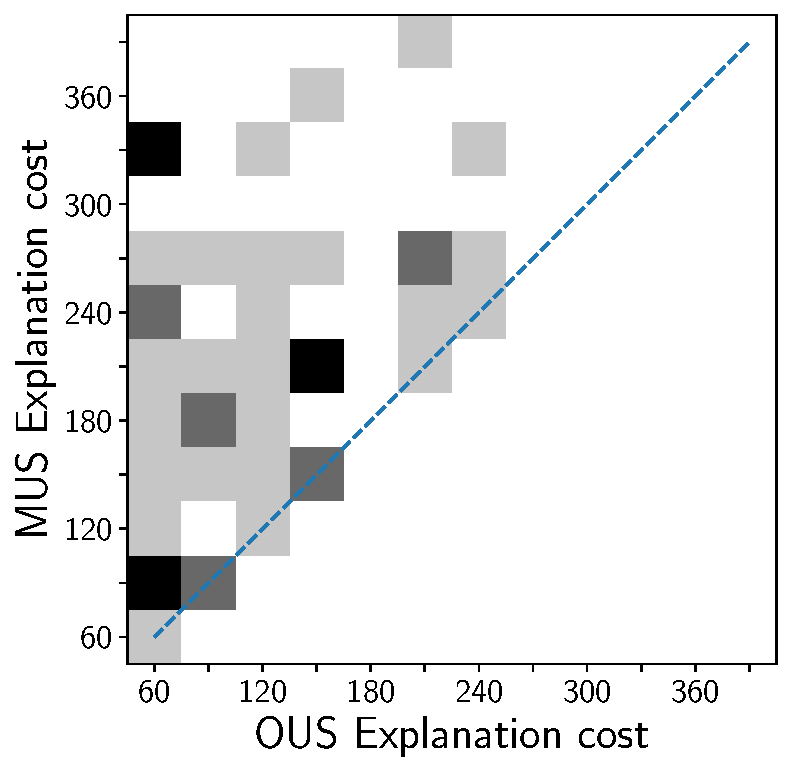
\includegraphics[width=0.5\columnwidth]{figures/heatmap_costs_mus_cous.pdf}
	\caption{Q1 - Explanation quality comparison of optimal versus subset-minimal explanations in the generated puzzle explanation sequences.}
	\label{fig:rq1_heatmap}
\end{figure}


\subsection{RQ2. Domain-specific vs disj. mcs grow}

\subsection{RQ3. Effect of COnstrainedness on the time required to computed explanations}

\subsection{RQ4. Does re-use of information across the different iterations improve efficiency?}

\begin{figure}[!h]
	\begin{subfigure}{0.47\textwidth}
		\centering
		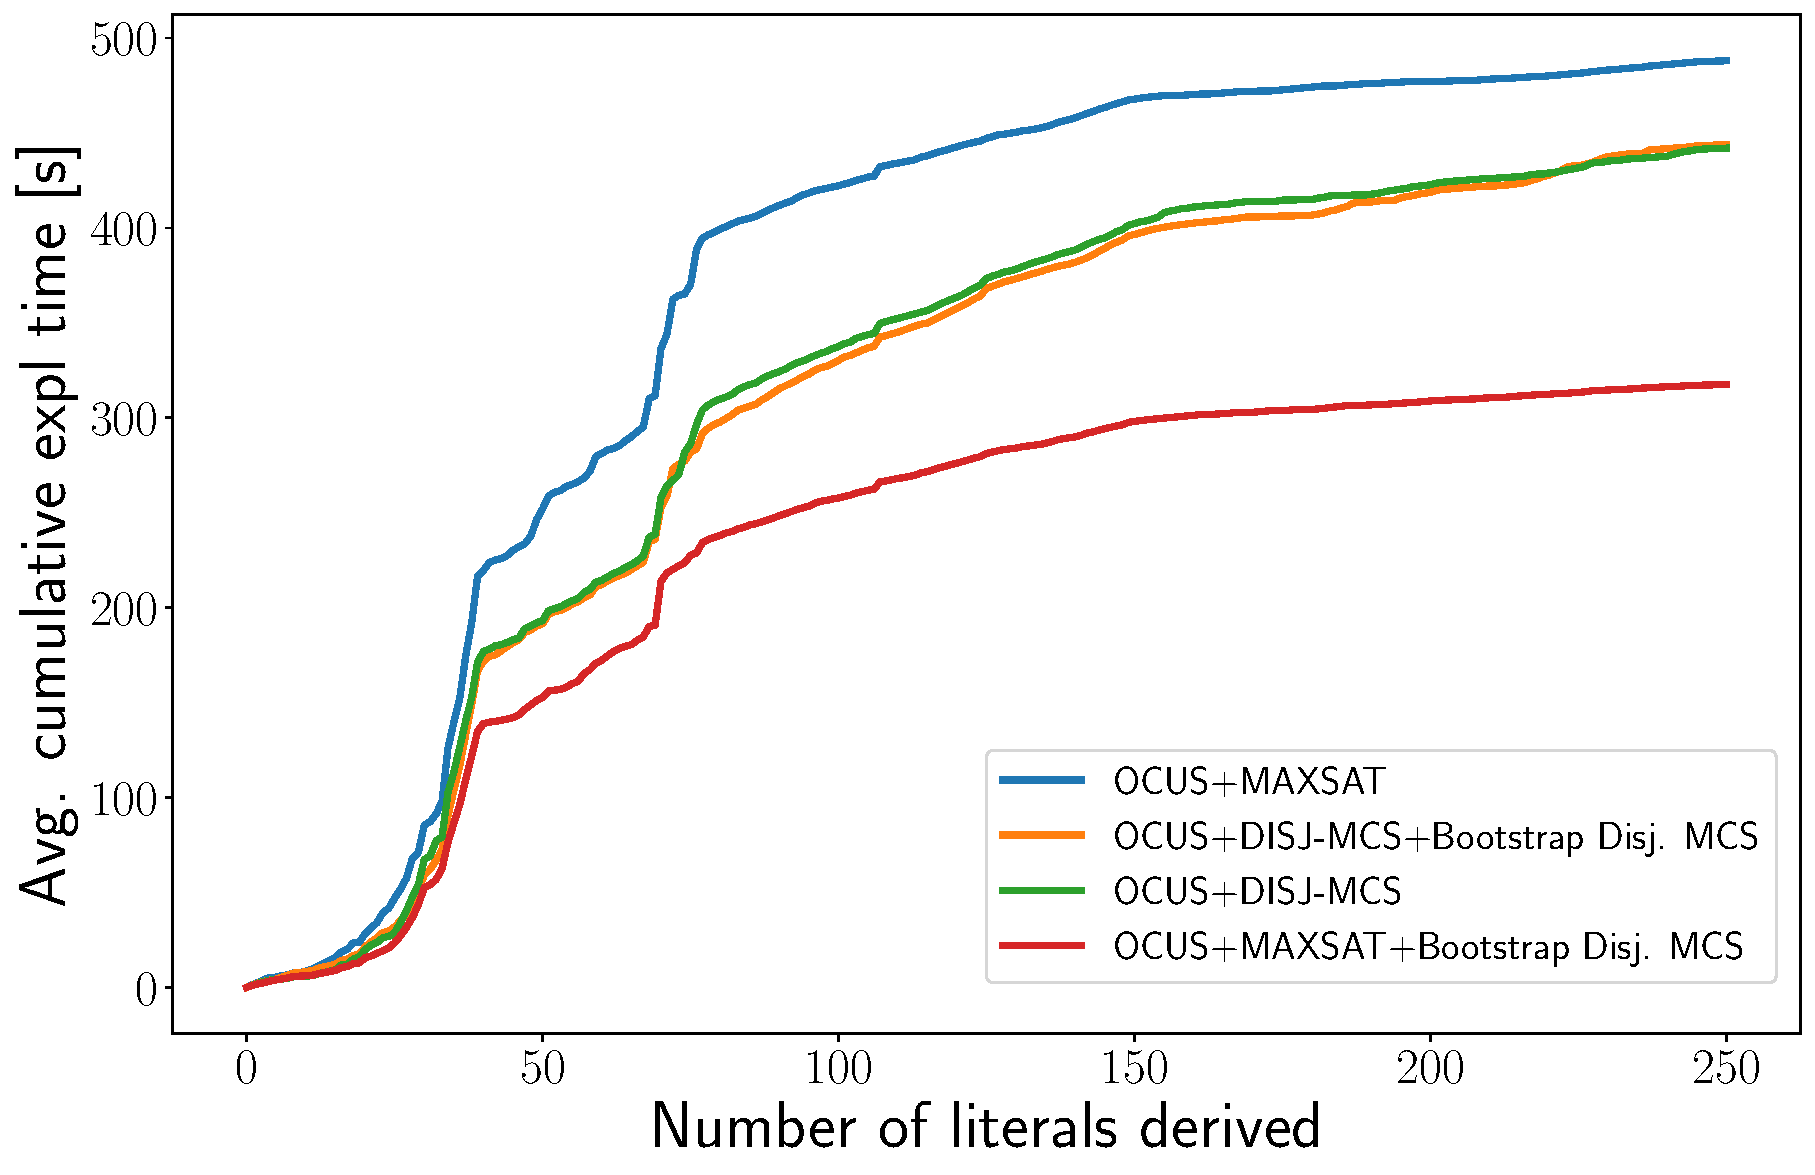
\includegraphics[width=\textwidth]{figures/ocus_disj_mcses.pdf}
		\label{fig:rq1_heatmap}
	\end{subfigure}
	\hfill
	\begin{subfigure}{0.47\textwidth}
		\centering
		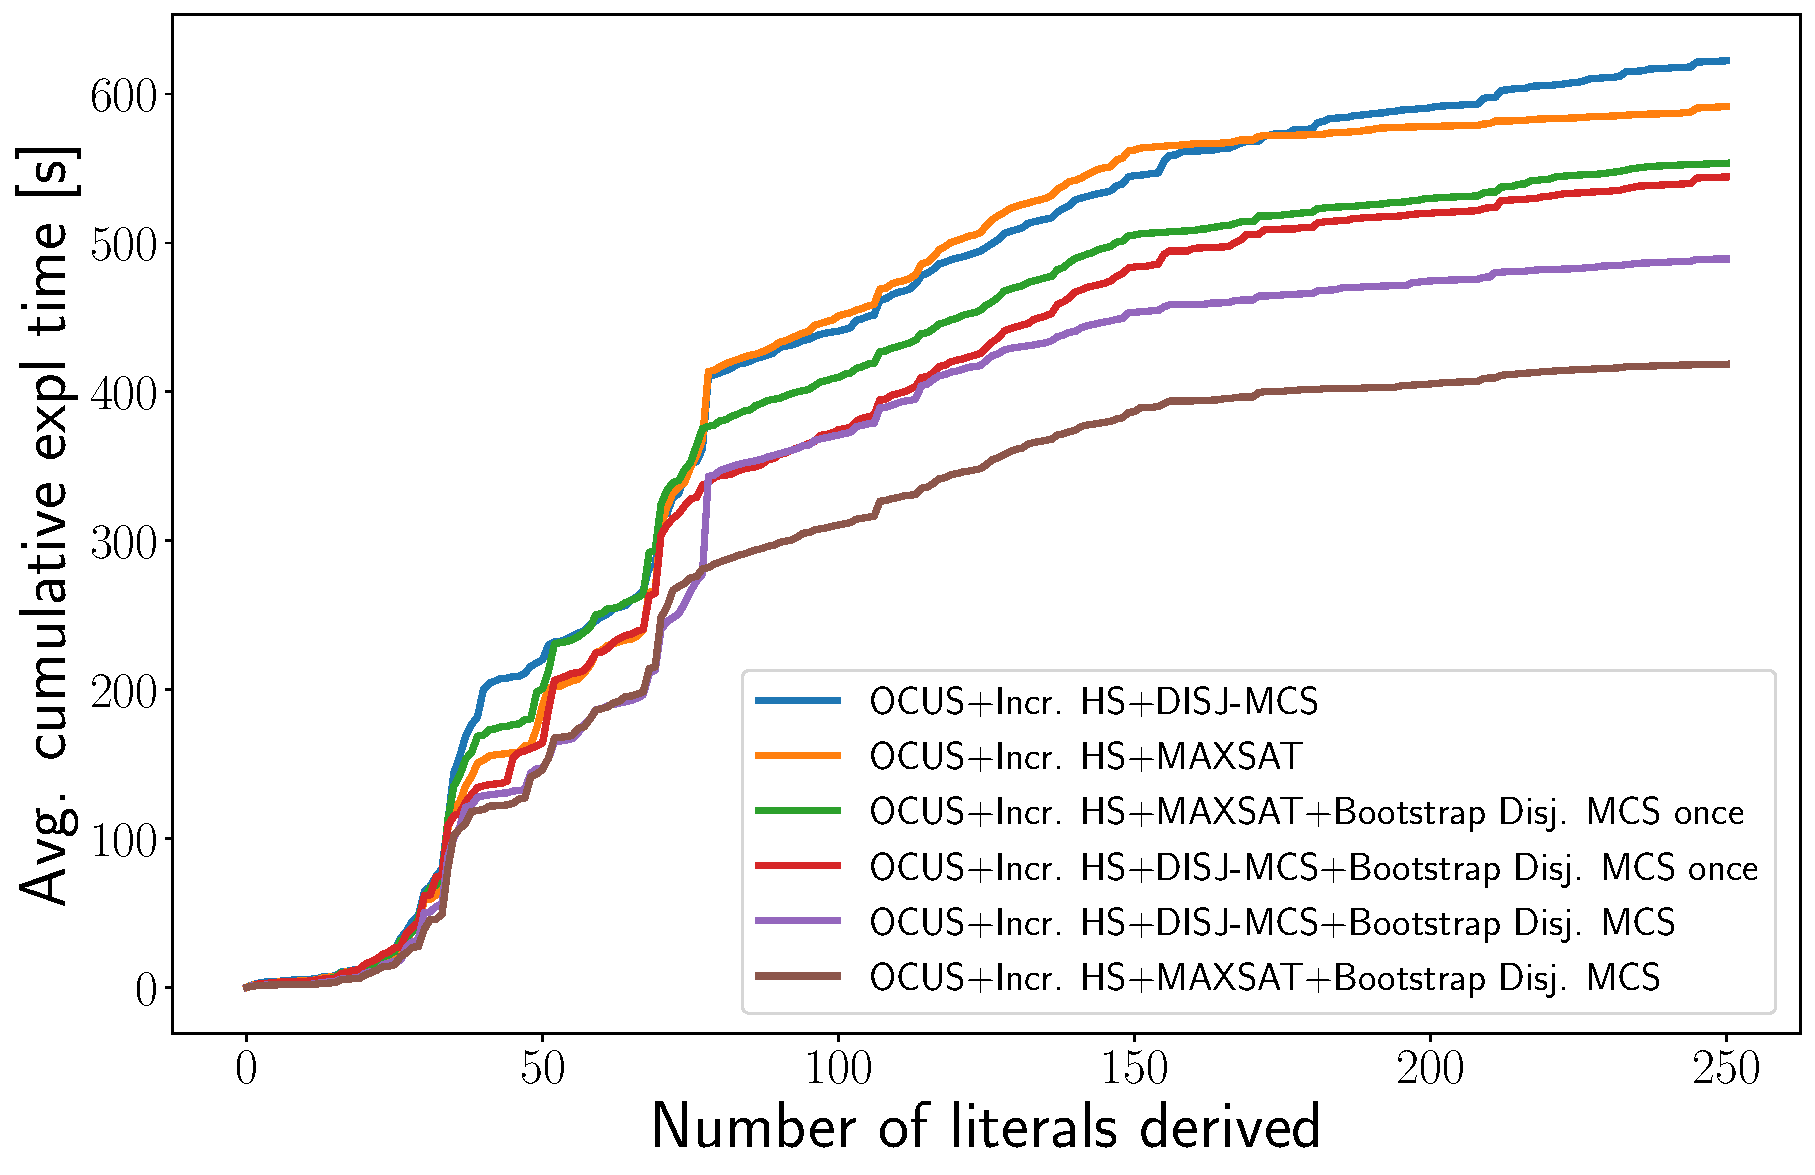
\includegraphics[width=\textwidth]{figures/ocus_incr_disj_mcses.pdf}
		\label{fig:rq1_heatmap}
	\end{subfigure}
\end{figure}

\subsection{RQ5. Does appropriate sorting of literals lead to faster generation of individual explanations and explanation sequences ?}

\begin{figure}[!h]
	\centering
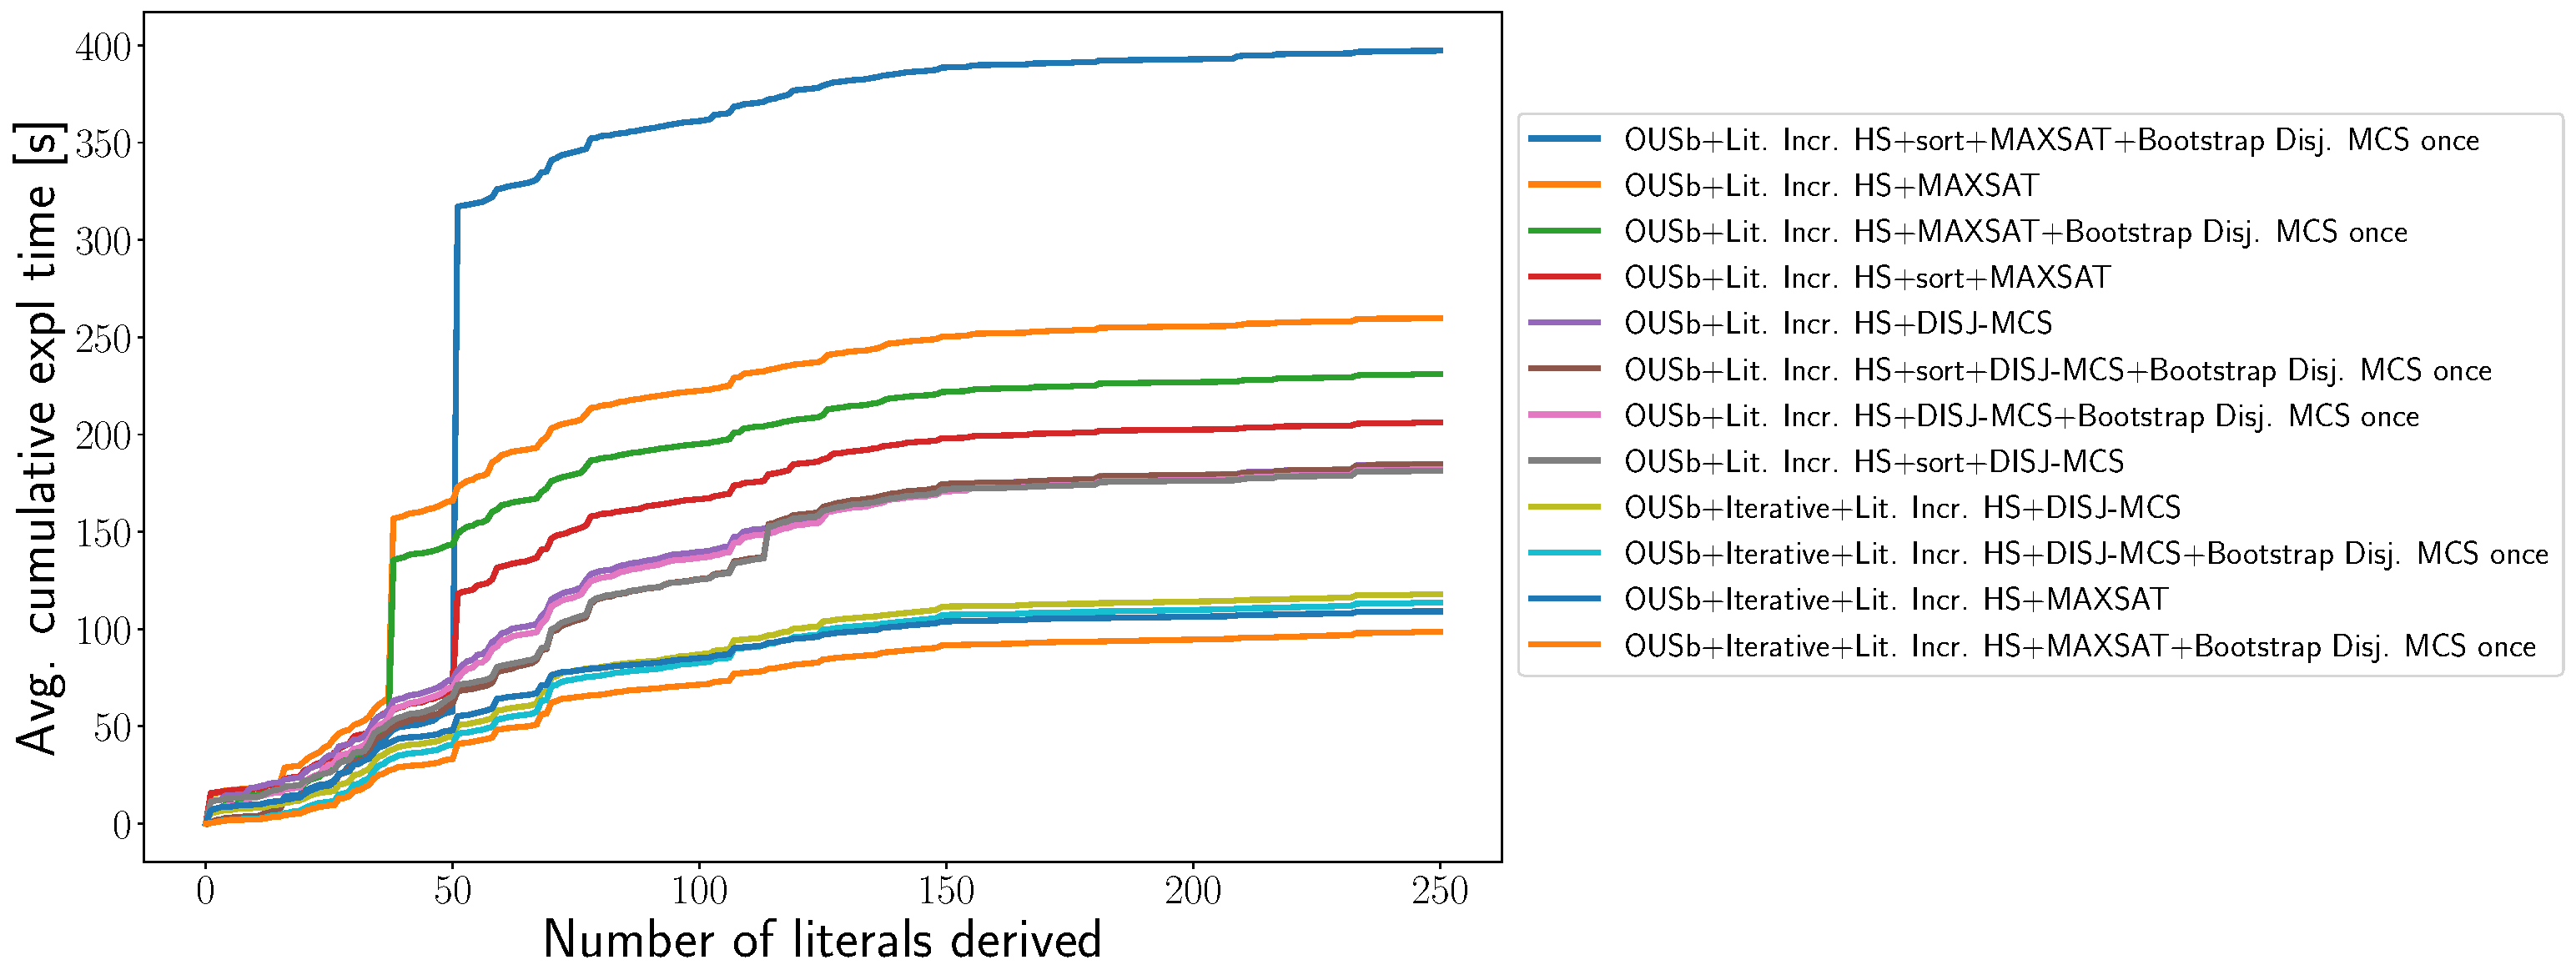
\includegraphics[width=\textwidth]{figures/ousb.pdf}
\label{fig:rq1_heatmap}
\end{figure}


% Graph of most important configurations
% 1) improvement with disjoint mcs enumeration
% 2) Replacing the grow with other strategies: DIJS MCSes
% 3) Replacing greedy loop with iterative search
% 4) Constrained

%\subsection{Hitting set computation}
% someway to present set coverage between hittingsets
% \number of hitting sets computed for the most important configuration
% 

\begin{figure}[!h]
\begin{subfigure}{0.45\textwidth}
	\centering
	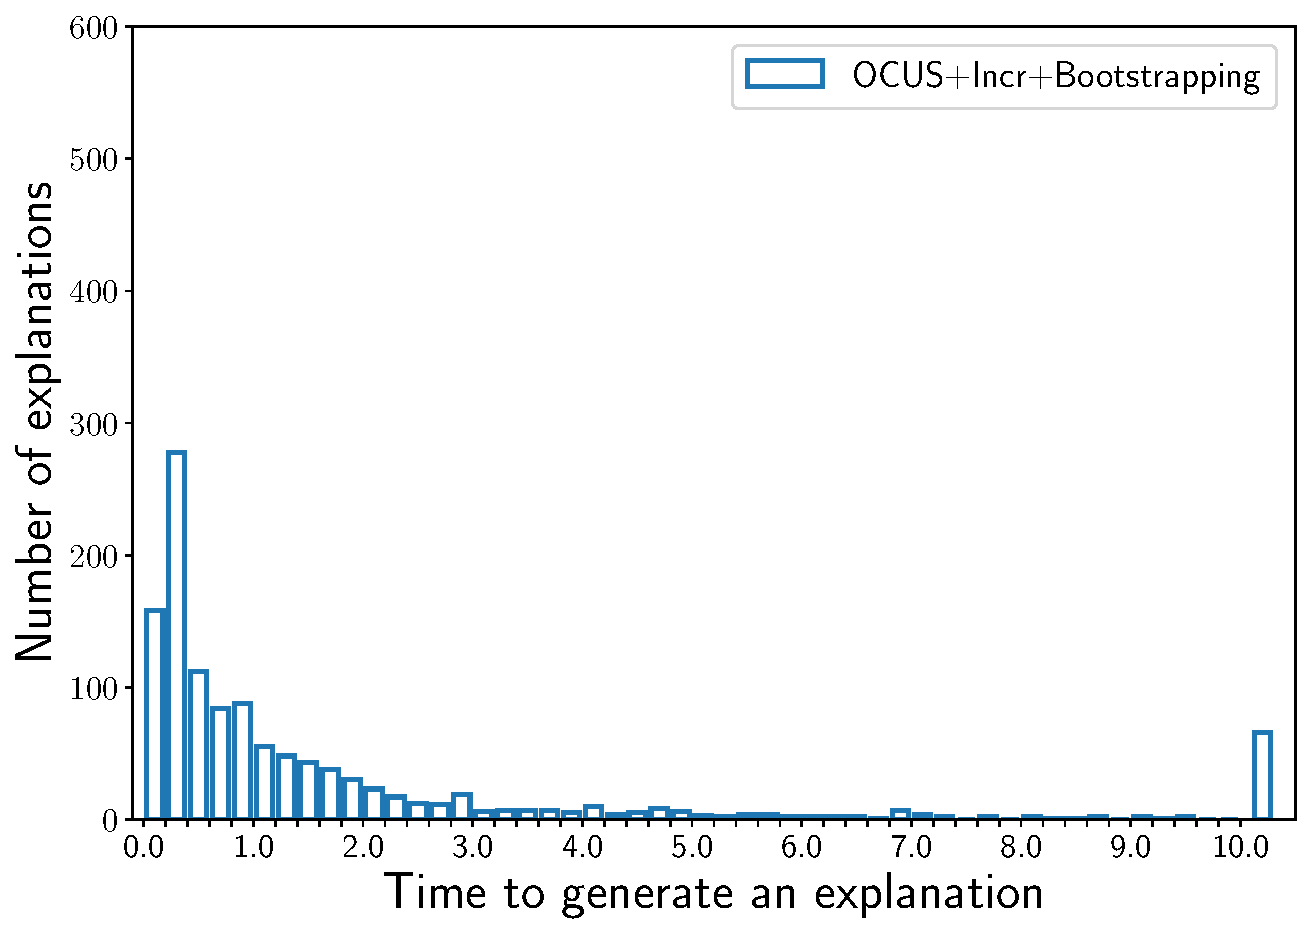
\includegraphics[width=\textwidth]{figures/explanation_times_histogram0.pdf}
	\caption{Incremental Constrained OUS with bootstrapping}
	\label{fig:first}
\end{subfigure}
\hfill
\begin{subfigure}{0.45\textwidth}
		\centering
	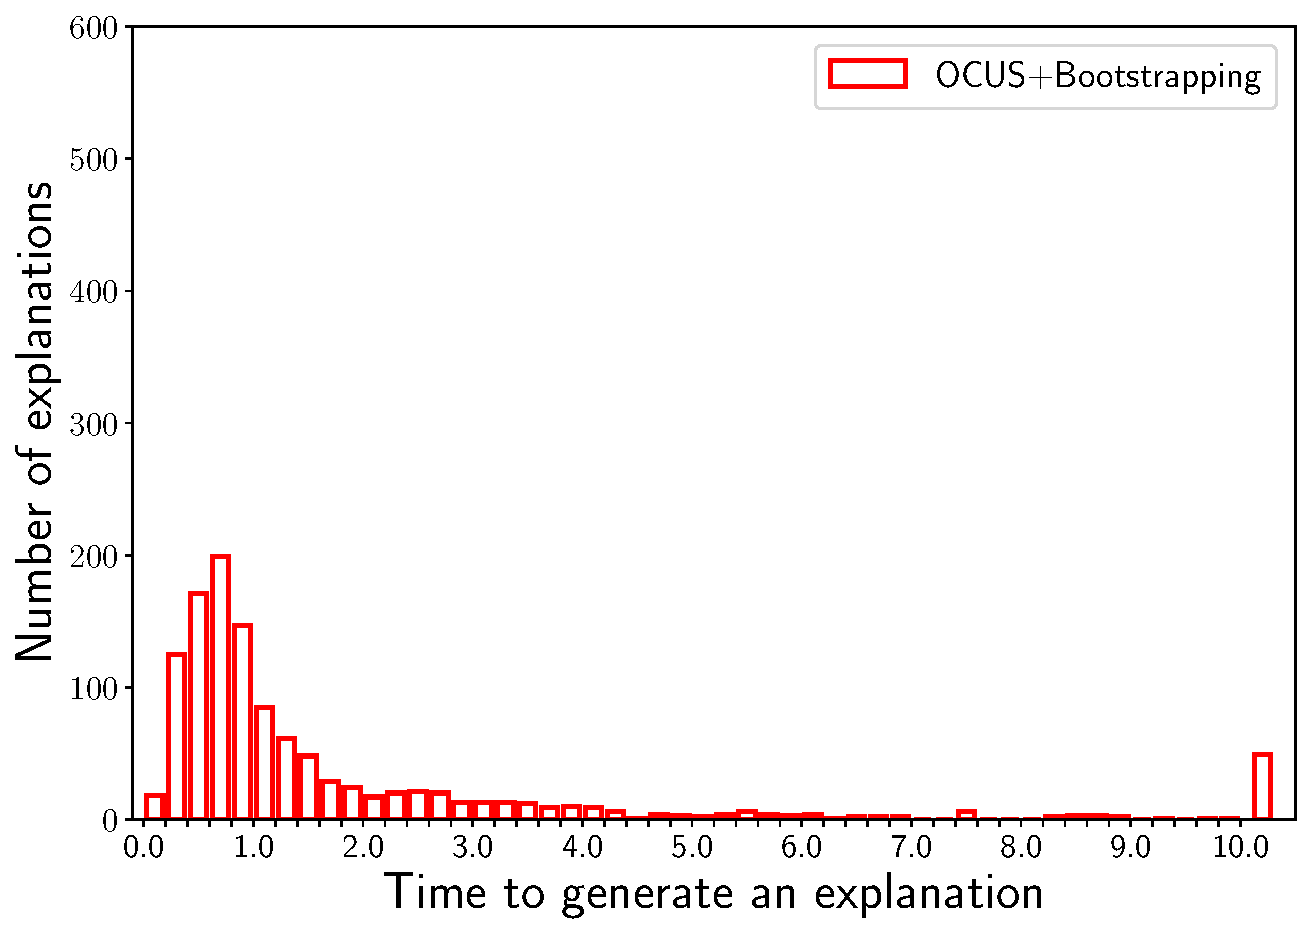
\includegraphics[width=\textwidth]{figures/explanation_times_histogram1.pdf}
	\caption{Incremental Constrained OUS with bootstrapping}
	\label{fig:second}
\end{subfigure}
\hfill
\begin{subfigure}{0.45\textwidth}
		\centering
	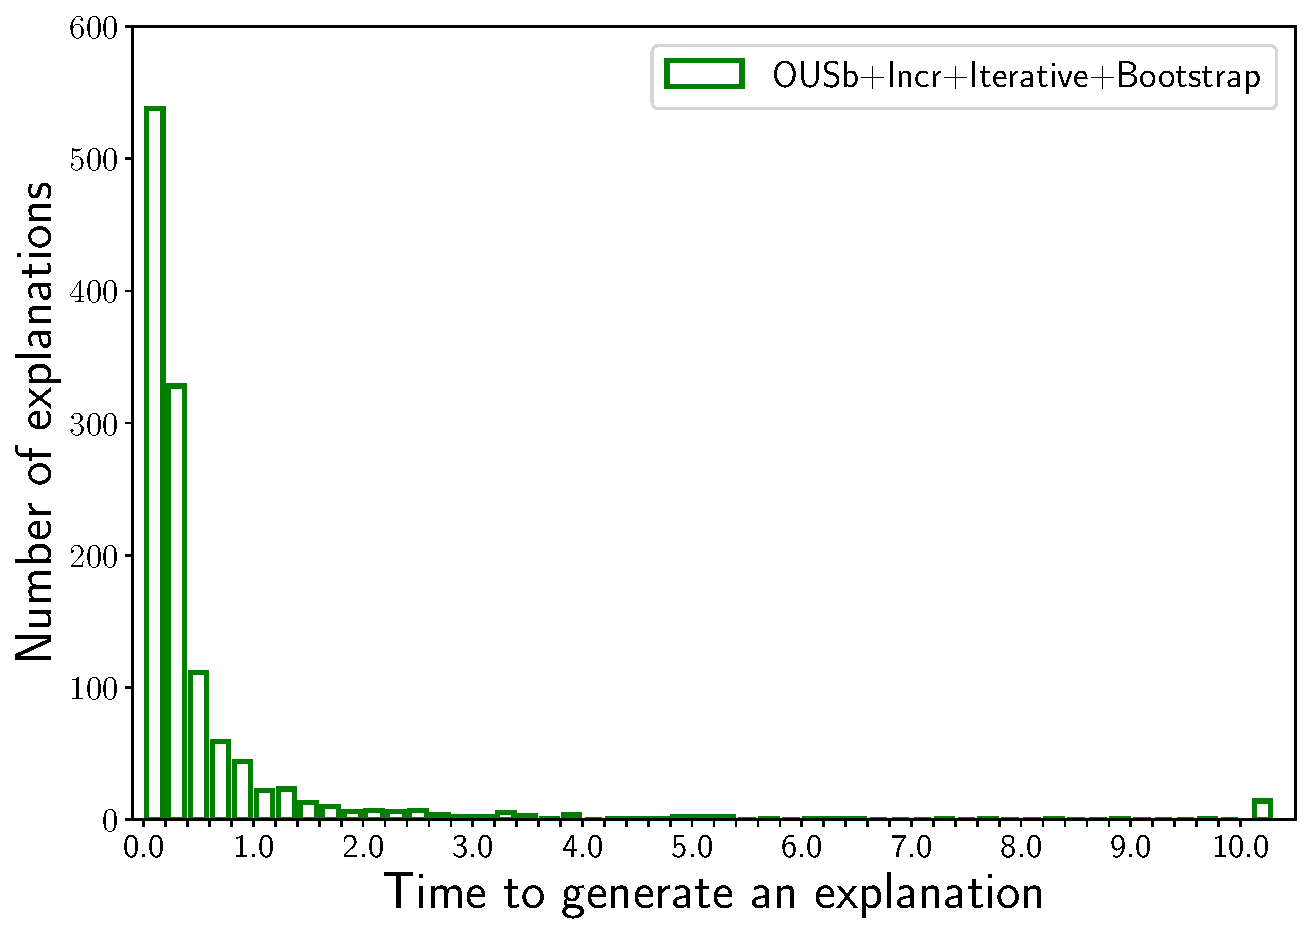
\includegraphics[width=\textwidth]{figures/explanation_times_histogram2.pdf}
	\caption{Incremental bounded OUS with disj. mcs enum. grow}
	\label{fig:third}
\end{subfigure}
\hfill
\begin{subfigure}{0.45\textwidth}
		\centering
	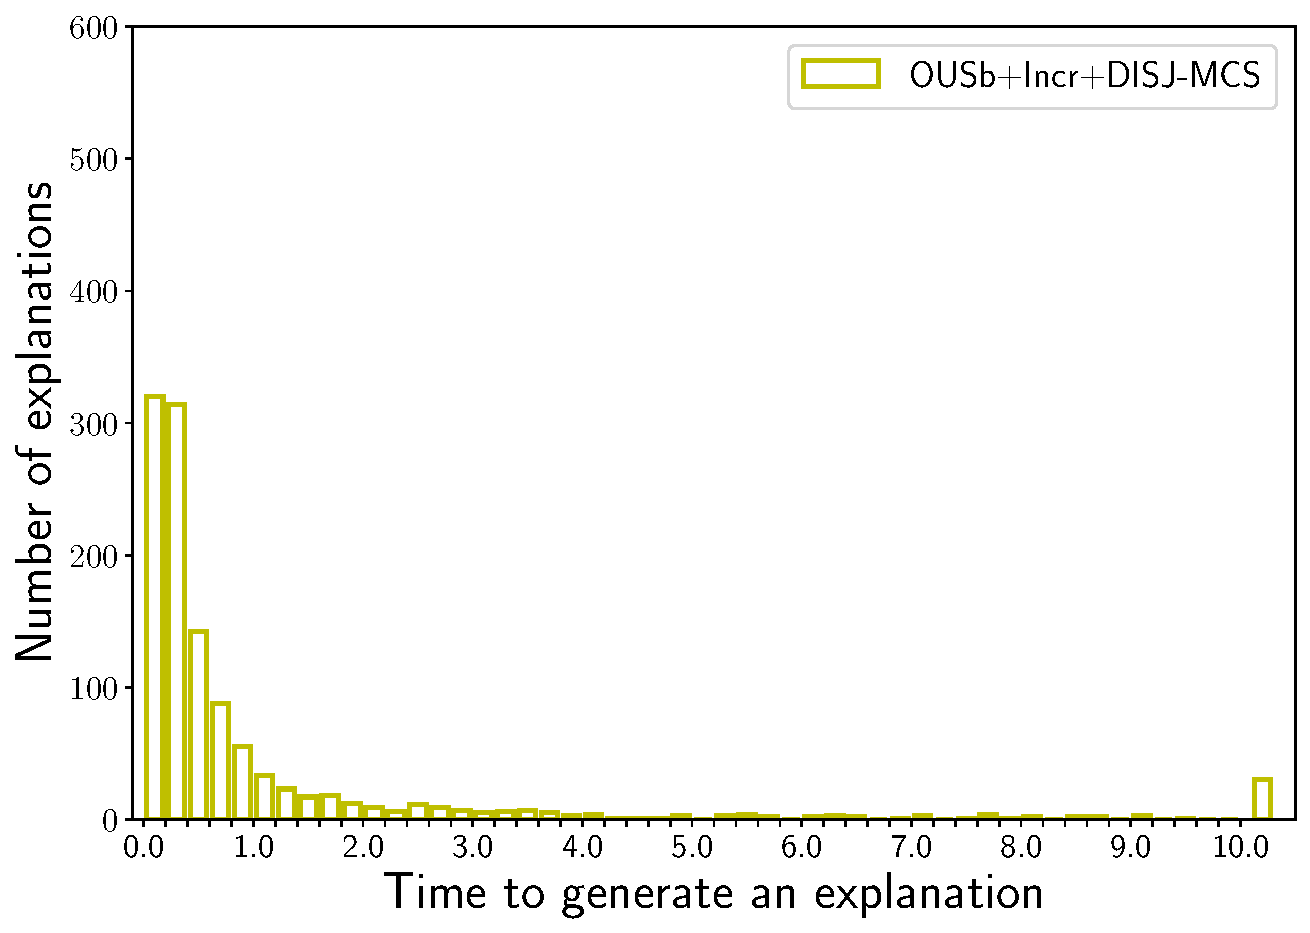
\includegraphics[width=\textwidth]{figures/explanation_times_histogram3.pdf}
	\caption{Iterative incremental bounded OUS with bootstrapping}
	\label{fig:third}
\end{subfigure}


\caption{Distribution of explanation generation time}
\label{fig:figures}

\end{figure}

\section{Conclusion and Future work}


\acks{Thanks!!}

\appendix
\section*{Appendix A.}

\vskip 0.2in
\bibliography{krrlib,ref}
\bibliographystyle{theapa}

\end{document}






